\documentclass{ctexrep}
\usepackage[T1]{fontenc}
\usepackage[a4paper,top=1.5cm,bottom=1.5cm,left=2cm,right=2cm,marginparwidth=1.75cm]{geometry}
\usepackage{mathtools}
\usepackage{tikz}
\usepackage{booktabs}
\usepackage{caption}
\usepackage{outlines}
\usepackage{graphicx}
\usepackage{amsthm}
\usepackage{tabu}
\usepackage{minted}
\usepackage[final]{pdfpages}
\usepackage[colorlinks=false, allcolors=blue]{hyperref}
\usepackage{cleveref}
\usepackage{psql}
% \usepackage{markdown}
\usepackage{underscore}
\usepackage{longtable}
\usepackage{csquotes}
\renewcommand{\tableautorefname}{表}
\DeclarePairedDelimiter{\set}{\{}{\}}
\DeclarePairedDelimiter{\paren}{(}{)}
\graphicspath{ {./images/} }
\newcommand*{\fullref}[1]{
\ifthenelse{\equal{\thepage}{\getpagerefnumber{#1}}}
  {
    \hyperref[{#1}]{\Cref*{#1} \nameref*{#1}}
  }
  {% false case
    \hyperref[{#1}]{第 \pageref*{#1} 页 \Cref*{#1} \nameref*{#1}}
  }
}
\definecolor{bg}{rgb}{0.95,0.95,0.95}

\newmintinline[sql]{postgresql}{}

% \title{标题}
% \author{卢雨轩 19071125}
% \date{\today}
\ctexset{
    chapter = {
        titleformat = \raggedright,
        name = {实验,:},
        number = \chinese{chapter}
    },
    section = {
        titleformat = \raggedright,
        name = {,},
        number = \chinese{section}、
    },
    paragraph = {
        runin = false
    },
    today = small,
    figurename = 图,
    contentsname = 目录,
    tablename = 表,
}

\begin{document}

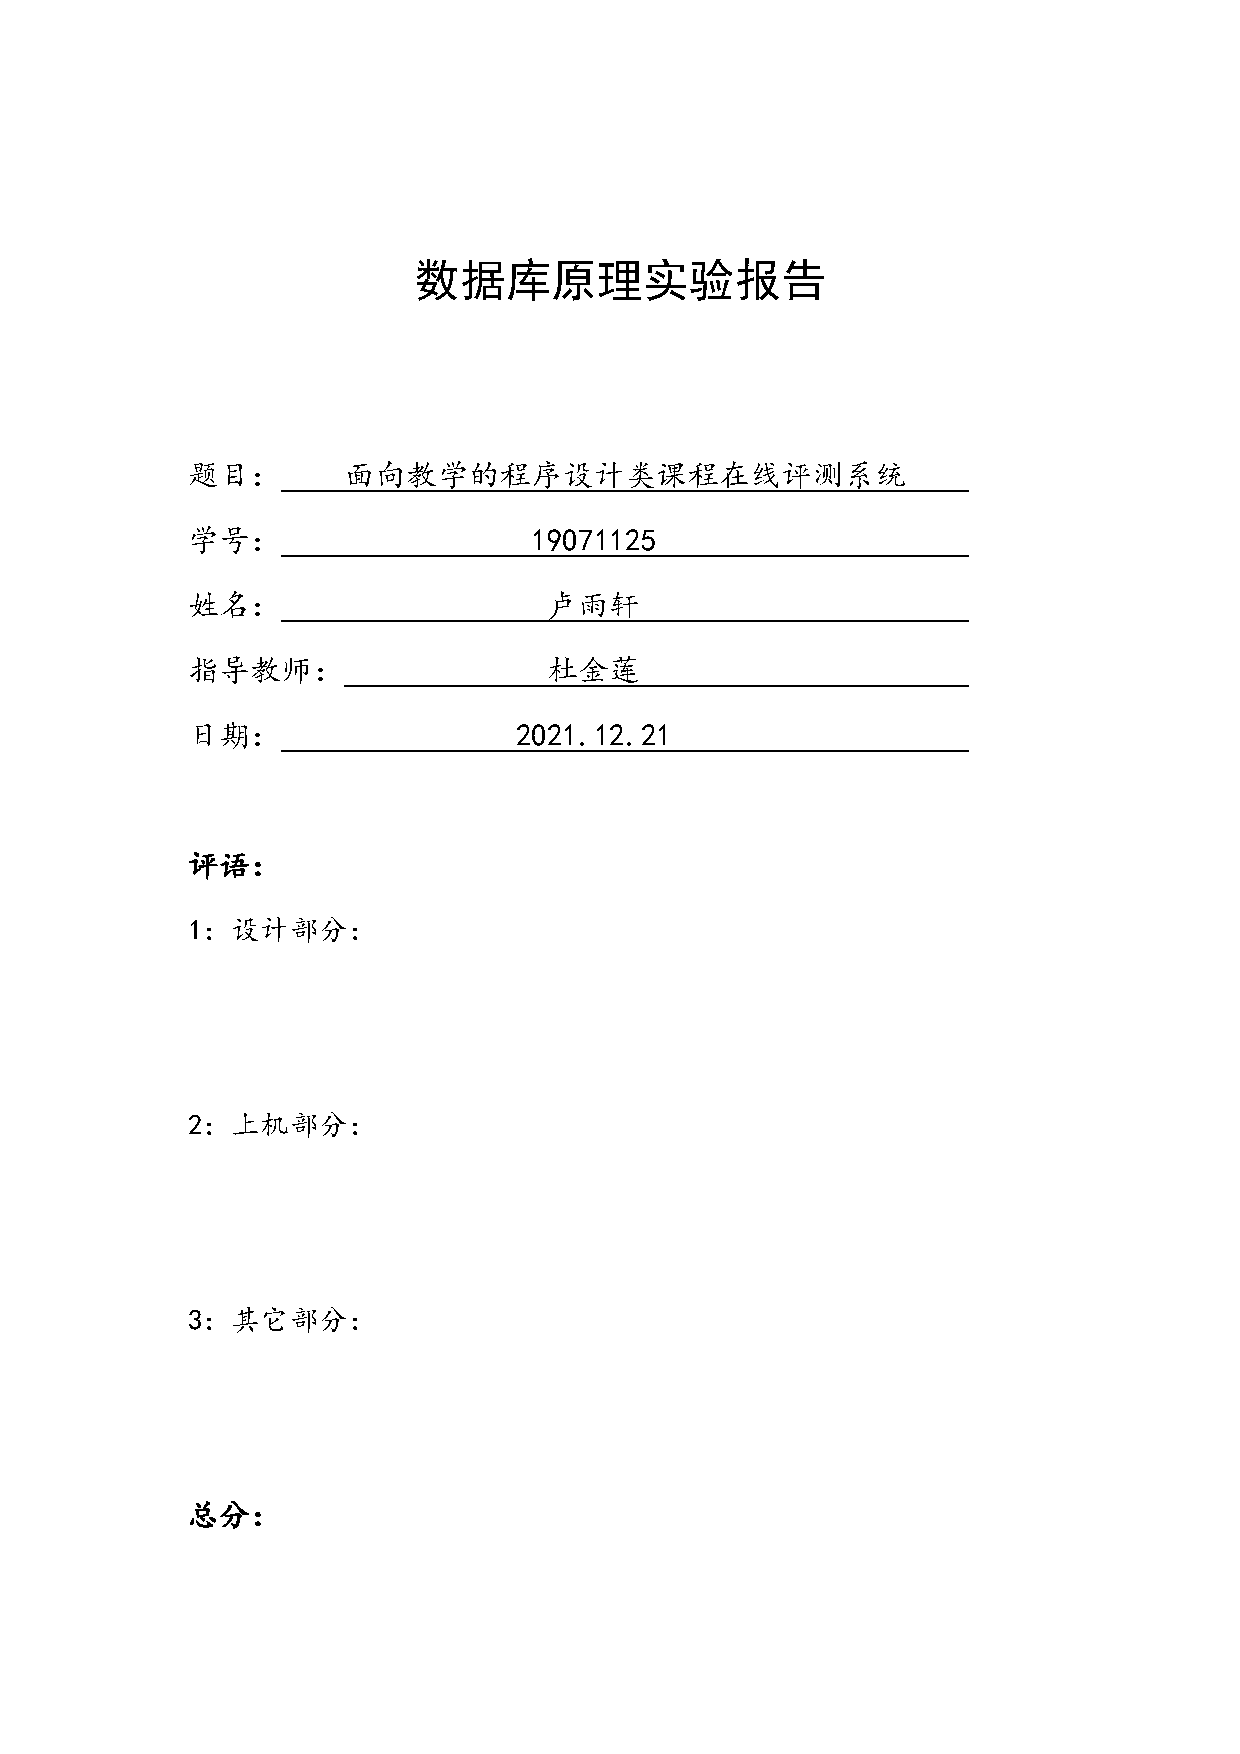
\includepdf{report-cover.pdf}

\tableofcontents
\clearpage
\chapter*{相关说明}
\section*{实验环境:}
PostgreSQL版本:\texttt{psql (PostgreSQL) 12.9 (Ubuntu 12.9-0ubuntu0.20.04.1)}

openGauss版本:\texttt{gsql (openGauss 2.0.0 build 78689da9)}

\section*{数据库设计}

本实验涉及的数据库设计源自\href{https://github.com/EduOJ/backend}{EduOJ}后端数据库的用户、权限、班级管理部分。\href{https://github.com/EduOJ/backend}{EduOJ}的数据库设计由卢雨轩(本实验报告的作者)和孙天天共同完成。复用以往项目作为实验设计的行为已经经过指导老师授权。

\chapter*{数据库设计}

\section{数据需求描述}

\subsection{管理员:}

\begin{itemize}
\item
  用户增删改查
\item
  班级增删改查
\item
  作业增删改查
\item
  成绩查询、修改
\end{itemize}

\hypertarget{ux7528ux6237ux76f8ux5173}{%
\subsubsection{用户相关}\label{ux7528ux6237ux76f8ux5173}}

\begin{itemize}
\item
  姓名,学号,密码,邮箱
\item
  权限相关:

  \begin{itemize}
  \item
    『全局权限』(如:某个用户有权限创建用户、修改用户、创建班级、创建题目)
  \item
    『针对权限』(如:某个用户有针对id为5的班级的添加学生权限)
  \item
    希望能够『批量管理』:把权限授予给『角色』,让『用户』拥有『角色』。
  \end{itemize}
\item
  统计信息,加快查询速度
\end{itemize}

\subsubsection{班级相关}

\begin{itemize}
\item
  课程名称,课堂名称,管理老师,课程描述
\item
  用户、作业

  \begin{itemize}
  \item
    和用户是多对多关系
  \item
    和作业是多对多关系
  \end{itemize}
\end{itemize}

\hypertarget{ux4f5cux4e1aux76f8ux5173}{%
\subsubsection{作业相关}\label{ux4f5cux4e1aux76f8ux5173}}

\begin{itemize}
\item
  标题,起止日期
\item
  多道题目
\item
  统计成绩
\end{itemize}

\hypertarget{ux6210ux7ee9ux67e5ux8be2ux4feeux6539}{%
\subsubsection{成绩查询、修改}\label{ux6210ux7ee9ux67e5ux8be2ux4feeux6539}}

\begin{itemize}
\item
  用户、班级、作业、成绩
\item
  根据用户做题记录生成,用于加快计算,\textbf{有数据冗余}。
\end{itemize}

\section{数据库设计}


\subsection{ER图}

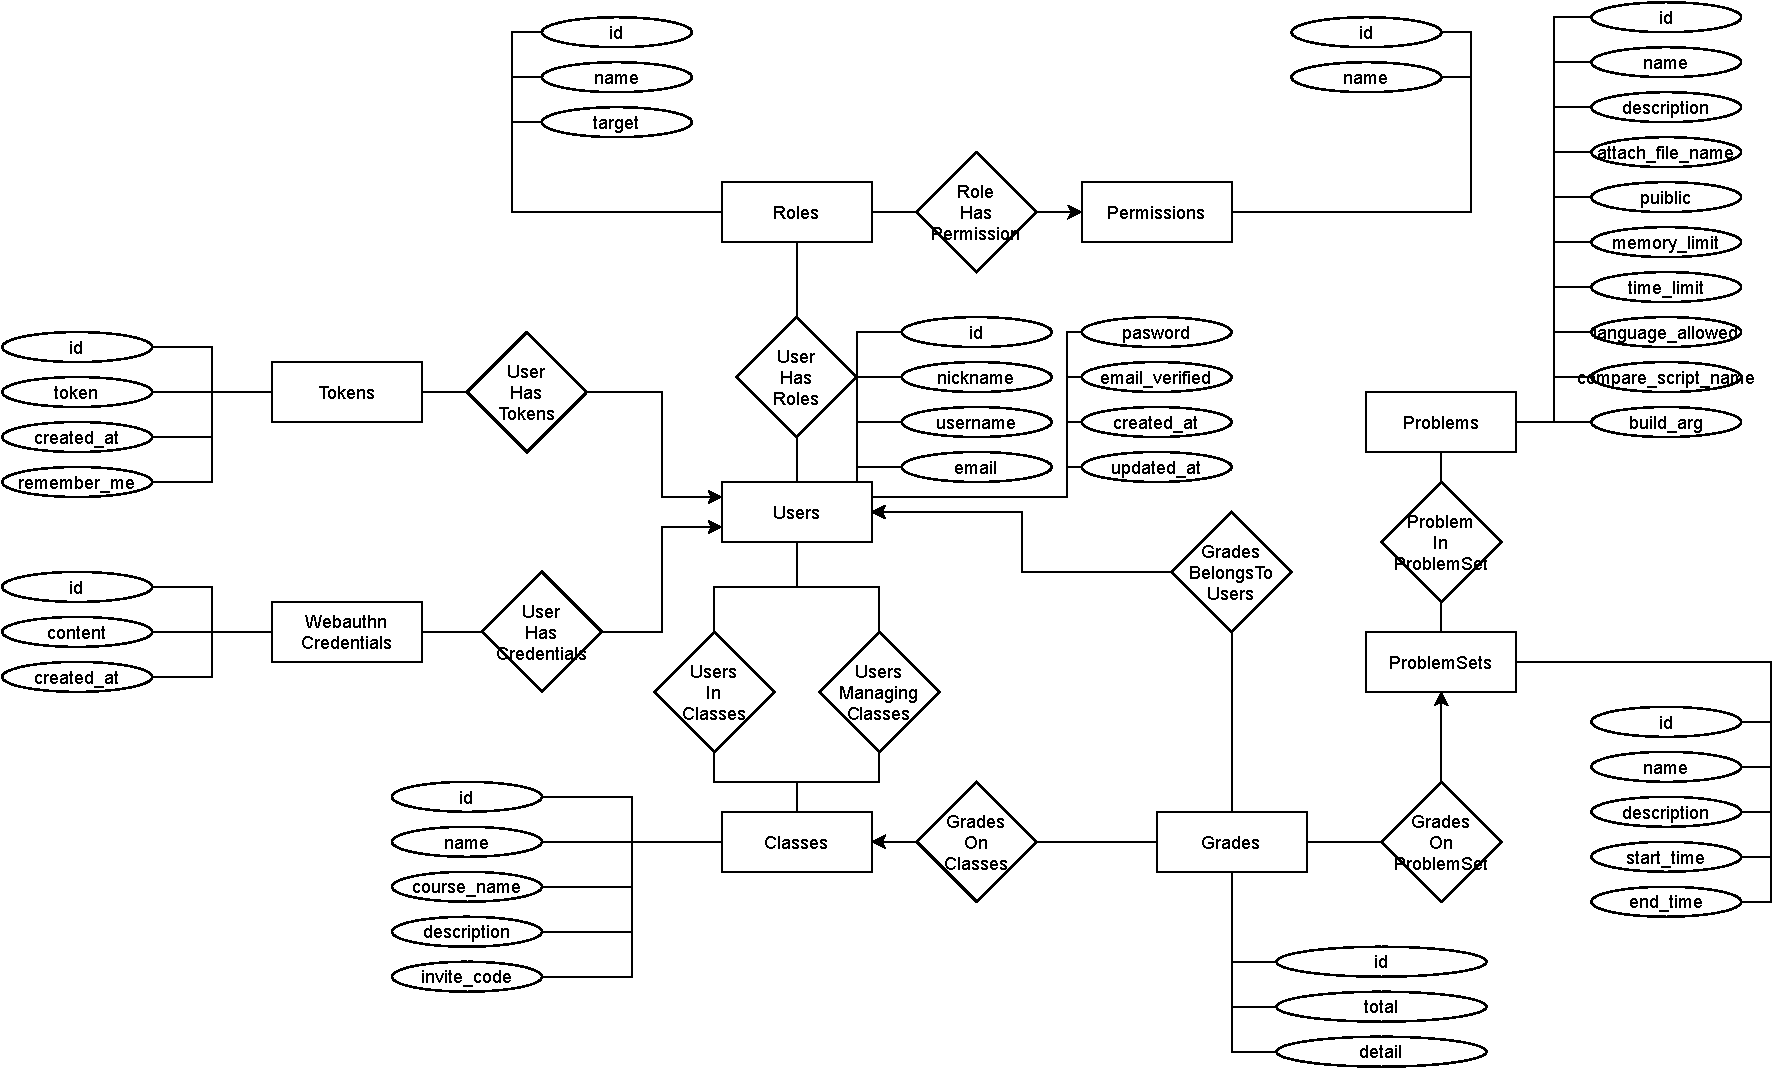
\includegraphics[width=\linewidth]{./course-design-er.pdf}
\captionof{figure}{EduOJ用户、班级、作业、权限管理部分ER图}


\subsection{关系模式}

\begin{itemize}
\item
  user(\underline{id}, nickname, username, email, password, created_at, updated_at)
\item
  roles(\underline{id}, name, target)
\item
  user_has_roles(\underline{id}, user_id, )
\item
  permissions(\underline{id},role_id, name)
\item
  tokens(\underline{id},user_id,token, created_at,remember_me)
\item
  webauthn_credentials(\underline{id}, user_id, content, created_at)
\item
  classes(\underline{id}, name, course_name, description, invite_code)
\item
  user_in_classes(\underline{id}, user_id, class_id)
\item
  user_managing_classes(\underline{id}, user_id, class_id)
\item
  grades(\underline{id}, total, detail, user_id, class_id,
  problem_set_id)
\item
  problem_sets(\underline{id}, name, description,
  start_time,end_time)
\item
  problem_in_problem_sets(\underline{id}, problem_id,
  problem_set_id)
\item
  problems(\underline{id}, name, description, attach_file_name,
  public, memory_limit, time_limit, compare_script_name, build_arg)
\end{itemize}


\subsection{范式判断}


\subsubsection{1NF}

所有关系模式中,属性均是原子的,符合范式。

\subsubsection{2NF}

除了grades的所有关系模式中均依赖主键\underline{id},符合范式。

grades中,class_id依赖problem_set_id、detail和total依赖评测结果(未给出),但是为了加速查询,保留数据冗余。


\subsubsection{3NF}

表中除了主键之外所有属性均不互相依赖,符合范式。

\subsubsection{BCNF}

所有关系模式均只有一个主属性,不存在其他键码,同时非主属性也依赖与键码,所以符合范式。
\subsubsection{4NF}

所有关系模式均不存在平凡多值依赖,故符合4NF。

\section{数据表设计}

\subsection{users}

\begin{longtable}[]{@{}cccc@{}}
\toprule
字段名称 & 类型 & 索引 & 外键\tabularnewline
\midrule
id & bigint & primary &\tabularnewline
username & varchar(30) & index &\tabularnewline
nickname & varchar(30) & index &\tabularnewline
email & varchar(320) & index &\tabularnewline
password & varchar(60) & &\tabularnewline
created_at & timestamp & &\tabularnewline
updated_at & timestamp & &\tabularnewline
\bottomrule
\end{longtable}

\subsubsection{roles}

\begin{longtable}[]{@{}cccc@{}}
\toprule
字段名称 & 类型 & 索引 & 外键\tabularnewline
\midrule
id & bigint & primary &\tabularnewline
name & varchar(255) & &\tabularnewline
target & varchar(255) & index &\tabularnewline
\bottomrule
\end{longtable}

\subsubsection{user_has_roles}



\begin{longtable}[]{@{}cccc@{}}
\toprule
字段名称 & 类型 & 索引 & 外键\tabularnewline
\midrule
id & bigint & primary &\tabularnewline
user_id & bigint & index & users(id)\tabularnewline
role_id & bigint & index & roles(id)\tabularnewline
target_id & bigint & index &\tabularnewline
\bottomrule
\end{longtable}



\hypertarget{permissions}{%
\subsection{permissions}\label{permissions}}



\begin{longtable}[]{@{}cccc@{}}
\toprule
字段名称 & 类型 & 索引 & 外键\tabularnewline
\midrule
id & bigint & primary &\tabularnewline
role_id & bigint & index & roles(id)\tabularnewline
name & varchar(255) & index &\tabularnewline
\bottomrule
\end{longtable}


\subsection{tokens}



\begin{longtable}[]{@{}cccc@{}}
\toprule
字段名称 & 类型 & 索引 & 外键\tabularnewline
\midrule
id & bigint & primary &\tabularnewline
user_id & bigint & index & users(id)\tabularnewline
token & varchar(32) & index &\tabularnewline
created_at & timestamp & &\tabularnewline
remember_me & boolean & &\tabularnewline
\bottomrule
\end{longtable}


\subsection{webauthn_credentials}

\begin{longtable}[]{@{}cccc@{}}
\toprule
字段名称 & 类型 & 索引 & 外键\tabularnewline
\midrule
id & bigint & primary &\tabularnewline
user_id & bigint & index & users(id)\tabularnewline
content & varchar(32) & &\tabularnewline
created_at & timestamp & &\tabularnewline
\bottomrule
\end{longtable}

\subsection{classes}


\begin{longtable}[]{@{}cccc@{}}
\toprule
字段名称 & 类型 & 索引 & 外键\tabularnewline
\midrule
id & bigint & primary &\tabularnewline
name & varchar(255) & &\tabularnewline
course_name & varchar(255) & &\tabularnewline
description & text & &\tabularnewline
invite_code & varchar(255) & index &\tabularnewline
\bottomrule
\end{longtable}


\subsection{user_in_classes}



\begin{longtable}[]{@{}cccc@{}}
\toprule
字段名称 & 类型 & 索引 & 外键\tabularnewline
\midrule
id & bigint & primary &\tabularnewline
user_id & bigint & index & users(id)\tabularnewline
class_id & bigint & index & classes(id)\tabularnewline
\bottomrule
\end{longtable}


\subsection{user_managing_classes}



\begin{longtable}[]{@{}cccc@{}}
\toprule
字段名称 & 类型 & 索引 & 外键\tabularnewline
\midrule
id & bigint & primary &\tabularnewline
user_id & bigint & index & users(id)\tabularnewline
class_id & bigint & index & classes(id)\tabularnewline
\bottomrule
\end{longtable}


\subsection{grades}



\begin{longtable}[]{@{}cccc@{}}
\toprule
字段名称 & 类型 & 索引 & 外键\tabularnewline
\midrule
id & bigint & primary &\tabularnewline
total & bigint & &\tabularnewline
detail & JSON & &\tabularnewline
user_id & bigint & index & users(id)\tabularnewline
class_id & bigint & index & classes(id)\tabularnewline
\bottomrule
\end{longtable}


\subsection{problem_sets}



\begin{longtable}[]{@{}cccc@{}}
\toprule
字段名称 & 类型 & 索引 & 外键\tabularnewline
\midrule
id & bigint & primary &\tabularnewline
class_id & bigint & index & classes(id)\tabularnewline
name & varchar(255) & &\tabularnewline
description & text & &\tabularnewline
start_time & timestamp & &\tabularnewline
end_time & timestamp & &\tabularnewline
created_at & timestamp & &\tabularnewline
updated_at & timestamp & &\tabularnewline
\bottomrule
\end{longtable}


\subsection{problem_in_problem_sets}



\begin{longtable}[]{@{}cccc@{}}
\toprule
字段名称 & 类型 & 索引 & 外键\tabularnewline
\midrule
id & bigint & primary &\tabularnewline
problem_id & bigint & index & problems(id)\tabularnewline
problem_set_id & bigint & index & problem_sets(id)\tabularnewline
\bottomrule
\end{longtable}

\subsection{problems}



\begin{longtable}[]{@{}cccc@{}}
\toprule
字段名称 & 类型 & 索引 & 外键\tabularnewline
\midrule
id & bigint & primary &\tabularnewline
name & varchar(255) & &\tabularnewline
description & text & &\tabularnewline
attach_file_name & varchar(255) & &\tabularnewline
public & boolean & &\tabularnewline
memory_limit & bigint & &\tabularnewline
time_limit & bigint & &\tabularnewline
build_arg & varchar(2047) & &\tabularnewline
compare_script_name & text & &\tabularnewline
\bottomrule
\end{longtable}



% \chapter*{数据库设计}

\chapter{创建和删除数据库}
\newcommand{\pgdb}{postgres}
\section{实验目的}
本实验要求使用这两种方法SQL语句创建和删除数据库,实验目的在于:
\begin{outline}[enumerate]
    \1 学习使用SQL语句建立与管理数据库。
    \1 学会SQL语句的排错技术。
    \1 了解数据文件、日志文件等相关概念。
    \1 建立案例数据库以及自己设计的数据库,为以后的实验做准备。
    \1 对常见错误操作,进行测试,加深对数据库管理相关语句以及操作的理解。
\end{outline}
\section{实验步骤}
\subsection{新建数据库}
\subsubsection{查看当前数据库情况}
使用\sql{\l}命令查看当前数据库情况,运行结果如下所示:
\begin{run}
\l
\end{run}
\subsubsection{使用SQL语句创建数据库}
\begin{runsilent}
    drop database if exists dbexp;
\end{runsilent}
使用 \sql{create database} 命令创建数据库,运行结果如下所示:
\begin{run}
    create database dbexp;
\end{run}
\subsubsection{观察数据库变化}
使用\sql{\l}命令查看当前数据库情况,运行结果如下所示:
\begin{run}
\l
\end{run}
可以看到,增加了\texttt{dbexp}数据库。

\subsection{删除数据库}
\subsubsection{使用SQL语句删除数据库}
使用 \sql{drop database} 命令删除数据库,运行结果如下所示:
\begin{run}
    drop database dbexp;
\end{run}
\subsubsection{观察数据库变化}
使用\sql{\l}命令查看当前数据库情况,运行结果如下所示:
\begin{run}
\l
\end{run}
可以看到,删除了\texttt{dbexp}数据库。

\begin{runsilent}
    create database dbexp;
\end{runsilent}
\renewcommand{\pgdb}{dbexp}

\section{思考题}
\subsection*{数据库文件有哪些增长方式?}
\begin{outline}[enumerate]
    \1 按百分比增长(例如:每次增长10\%)。
    \1 按固定长度增长(例如:每次增长1MiB)。
\end{outline}
\subsection*{日志文件的作用是什么?}
记录数据库执行过的所有命令。可以根据日志文件诊断数据库或恢复数据库(如:当服务器意外断电时,可能数据库文件被破坏,此时可以用binlog来恢复数据库文件。)

\section{心得体会}

实验过程中,碰到的主要问题就是实验用的数据库用户(\texttt{dbtest})默认没有建立数据库的权限。需要执行 \sql|alter user dbtest CREATEDB;| 来授予权限。

\chapter{创建和删除基本表}
\section{实验目的}
本实验的学习目标在于熟练掌握数据库基本表的创建、修改和删除的方法,具体实验目的如下:
\begin{outline}[enumerate]
    \1 学会使用SQL语句创建、修改和删除表。
    \1 学会使用SQL语句设置常用的数据完整性约束,含主键约束、外键约束、空值约束、UNIQUE约束、默认值以及CHECK约束等。
    \1 学会使用系统存储过程查看基本表信息。
    \1 熟悉SQL的常用数据类型。
    \1 理解相关概念:基本表与三级结构、实体完整性、参照完整性、用户定义完整性、主键、外键、空值、默认值等。
    \1 建立案例数据库以及自己设计的数据库的相关基本表,为后面的实验做准备。
    \1 测试各种异常、错误情况,加深对表管理操作以及相关知识点的理解。
\end{outline}

\section{实验步骤}
\subsection{创建表}
\subsubsection{查询当前数据库情况}
使用 \sql{\dt} 命令查看当前数据库情况,运行结果如下所示:
\begin{run}
    \dt
\end{run}
\subsubsection{创建表}
使用 \sql|CREATE TABLE| 命令在默认的public schema中创建一个数据表,并增加主键约束:
\begin{run}
    CREATE TABLE "users" (
        "id" bigserial,
        "username" varchar(30) NOT NULL,
        "nickname" varchar(30) NOT NULL,
        "email" varchar(320) NOT NULL,
        "password" varchar(60) NOT NULL,
        "created_at" timestamptz NOT NULL,
        "updated_at" timestamptz NOT NULL,
        "deleted_at" timestamptz,
        PRIMARY KEY ("id"),
        UNIQUE ("username"),
        UNIQUE ("email")
    )
\end{run}
\subsubsection{查询当前数据库情况}
使用 \sql{\dt} 命令查看当前数据库情况,运行结果如下所示:
\begin{run}
    \dt
\end{run}
可以看到,新增了users表。
\subsection{修改表}
\subsubsection{查询当前数据表情况}
使用 \sql{select} 命令查看当前数据表情况,运行结果如下所示:

\begin{run}
    SELECT column_name as Name, data_type as Type, is_nullable as Nullable, column_default as Default FROM information_schema.columns WHERE table_schema = 'public' AND table_name = 'users';
\end{run}

\subsubsection{修改数据表}
使用 \sql{alter table} 命令修改数据表,运行结果如下所示:

\begin{run}
    alter table users add column "age" integer;
\end{run}

\subsubsection{查询修改后数据表情况}
使用 \sql{select} 命令查看修改后数据表情况,运行结果如下所示:

\begin{run}
    SELECT column_name as Name, data_type as Type, is_nullable as Nullable, column_default as Default FROM information_schema.columns WHERE table_schema = 'public' AND table_name = 'users';
\end{run}

可以看到,增加了age字段。

\subsection{删除表}
\subsubsection{查询当前数据库情况}
使用 \sql{\dt} 命令查看当前数据库情况,运行结果如下所示:

\begin{run}
    \dt
\end{run}

\subsubsection{删除数据表}
使用 \sql{drop} 命令删除数据表,运行结果如下所示:
\begin{run}
    drop table users;
\end{run}
\subsubsection{查询操作后数据库情况}
使用 \sql{\dt} 命令查看操作后数据库情况,运行结果如下所示:

\begin{run}
    \dt
\end{run}
可以看到,不存在任何数据表,删除成功。

\begin{runsilent}
    CREATE TABLE "users" (
        "id" bigserial,
        "username" varchar(30) NOT NULL,
        "nickname" varchar(30) NOT NULL,
        "email" varchar(320) NOT NULL,
        "password" varchar(60) NOT NULL,
        "created_at" timestamptz NOT NULL,
        "updated_at" timestamptz NOT NULL,
        "deleted_at" timestamptz,
        PRIMARY KEY ("id"),
        UNIQUE ("username"),
        UNIQUE ("email")
    )
\end{runsilent}

\subsection{创建外键约束}
创建班级表,并创建外键约束:
\begin{run}
    CREATE TABLE "classes" (
        "id" bigserial,
        "name" varchar(255) NOT NULL,
        "course_name" varchar(255) NOT NULL,
        "description" text DEFAULT '',
        "invite_code" varchar(255) NOT NULL DEFAULT '',
        "created_at" timestamptz,
        "updated_at" timestamptz,
        "deleted_at" timestamptz,
        PRIMARY KEY ("id")
    );

    CREATE TABLE "user_in_classes" (
        "class_id" bigint not null,
        "user_id" bigint not null,
        PRIMARY KEY ("class_id", "user_id"),
        CONSTRAINT "fk_user_in_classes_class" FOREIGN KEY ("class_id") REFERENCES "classes"("id"),
        CONSTRAINT "fk_user_in_classes_user" FOREIGN KEY ("user_id") REFERENCES "users"("id")
    );
\end{run}
\subsubsection{测试外键是否创建成功}
尝试插入一条违反外键约束的数据:
\begin{run}
    insert into user_in_classes (class_id, user_id) values (2, 2);
\end{run}
可以看到,系统阻止了非法数据插入,外键创建成功。
\subsubsection{创建非空和唯一约束}
已经在第一步中创建了非空和唯一约束。下面验证是否成功:
\begin{run}
    insert into users (username, nickname, email, password, created_at, updated_at, deleted_at) values (null, 'test', 'test@test.com', 'password', '2021-12-14 00:00:00', '2021-12-14 00:00:00', null);
    insert into users (username, nickname, email, password, created_at, updated_at, deleted_at) values ('test', 'test', 'test@test.com', 'password', '2021-12-14 00:00:00', '2021-12-14 00:00:00', null);
    insert into users (username, nickname, email, password, created_at, updated_at, deleted_at) values ('test', 'test', 'test@test.com', 'password', '2021-12-14 00:00:00', '2021-12-14 00:00:00', null);
    insert into users (username, nickname, email, password, created_at, updated_at, deleted_at) values ('test1', 'test', 'test@test.com', 'password', '2021-12-14 00:00:00', '2021-12-14 00:00:00', null);
\end{run}
\begin{runsilent}
    truncate table users cascade;
\end{runsilent}
可以看到,系统阻止了非法数据插入,非空和唯一约束创建成功。
\subsection{默认值}
使用 \sql{select} 命令查看当前数据表结构,运行结果如下所示:

\begin{run}
    SELECT column_name as Name, data_type as Type, is_nullable as Nullable, column_default as Default FROM information_schema.columns WHERE table_schema = 'public' AND table_name = 'users';
\end{run}

可以看到 \sql{id} 列的默认值为 \sql{users_id_seq} 序列的下一个值。

\subsection{check约束}
\begin{runsilent}
    truncate table users cascade;
\end{runsilent}
\begin{run}
    ALTER TABLE users ADD CONSTRAINT check_username_length CHECK (LENGTH(username) > 6);
\end{run}
\subsubsection{检查check约束}
尝试插入违反check约束的数据:
\begin{run}
    insert into users (username, nickname, email, password, created_at, updated_at, deleted_at) values ('testtest', 'testtest', 'test1@test.com', 'password', '2021-12-14 00:00:00', '2021-12-14 00:00:00', null);insert into users (username, nickname, email, password, created_at, updated_at, deleted_at) values ('test', 'test', 'test2@test.com', 'password', '2021-12-14 00:00:00', '2021-12-14 00:00:00', null);
\end{run}
可以看到运行失败,系统阻止了非法数据插入。
\begin{runsilent}
    truncate table users cascade;
    alter table users drop constraint check_username_length;
\end{runsilent}

\subsection{创建后续实验所需要的其他数据表}

\begin{run}
    CREATE TABLE "user_manage_classes" (
        "class_id" bigint,
        "user_id" bigint,
        PRIMARY KEY ("class_id", "user_id"),
        CONSTRAINT "fk_user_manage_classes_class" FOREIGN KEY ("class_id") REFERENCES "classes"("id"),
        CONSTRAINT "fk_user_manage_classes_user" FOREIGN KEY ("user_id") REFERENCES "users"("id")
    );
    
    CREATE TABLE "roles" (
        "id" bigserial,
        "name" text,
        "target" text,
        PRIMARY KEY ("id")
    );
    
    CREATE TABLE "permissions" (
        "id" bigserial,
        "role_id" bigint,
        "name" text,
        PRIMARY KEY ("id"),
        CONSTRAINT "fk_roles_permissions" FOREIGN KEY ("role_id") REFERENCES "roles"("id")
    );
    
    CREATE TABLE "tokens" (
        "id" bigserial,
        "token" text,
        "user_id" bigint,
        "remember_me" boolean,
        "created_at" timestamptz,
        "updated_at" timestamptz,
        PRIMARY KEY ("id"),
        CONSTRAINT "fk_tokens_user" FOREIGN KEY ("user_id") REFERENCES "users"("id")
    );
    
    CREATE TABLE "webauthn_credentials" (
        "id" bigserial,
        "user_id" bigint,
        "content" text,
        "created_at" timestamptz,
        PRIMARY KEY ("id"),
        CONSTRAINT "fk_users_credentials" FOREIGN KEY ("user_id") REFERENCES "users"("id")
    );
    
    CREATE TABLE "problem_sets" (
        "id" bigserial,
        "class_id" bigint NOT NULL,
        "name" varchar(255) NOT NULL,
        "description" text,
        "start_time" timestamptz,
        "end_time" timestamptz,
        "created_at" timestamptz,
        "updated_at" timestamptz,
        "deleted_at" timestamptz,
        PRIMARY KEY ("id"),
        CONSTRAINT "fk_classes_problem_sets" FOREIGN KEY ("class_id") REFERENCES "classes"("id"),
        CONSTRAINT "fk_problem_sets_class" FOREIGN KEY ("class_id") REFERENCES "classes"("id")
    );
    
    CREATE TABLE "grades" (
        "id" bigserial,
        "user_id" bigint,
        "problem_set_id" bigint,
        "class_id" bigint,
        "detail" JSON,
        "total" bigint,
        "created_at" timestamptz,
        "updated_at" timestamptz,
        PRIMARY KEY ("id"),
        CONSTRAINT "fk_grades_user" FOREIGN KEY ("user_id") REFERENCES "users"("id"),
        CONSTRAINT "fk_grades_problem_set" FOREIGN KEY ("problem_set_id") REFERENCES "problem_sets"("id"),
        CONSTRAINT "fk_grades_class" FOREIGN KEY ("class_id") REFERENCES "classes"("id"),
        CONSTRAINT "fk_problem_sets_grades" FOREIGN KEY ("problem_set_id") REFERENCES "problem_sets"("id"),
        CONSTRAINT "fk_users_grades" FOREIGN KEY ("user_id") REFERENCES "users"("id")
    );
    
    CREATE TABLE "scripts" (
        "name" text,
        "filename" text,
        "created_at" timestamptz,
        "updated_at" timestamptz,
        PRIMARY KEY ("name")
    );
    
    CREATE TABLE "problems" (
        "id" bigserial,
        "name" varchar(255) NOT NULL DEFAULT '',
        "description" text,
        "attachment_file_name" varchar(255) NOT NULL DEFAULT '',
        "public" boolean NOT NULL DEFAULT false,
        "privacy" boolean NOT NULL DEFAULT false,
        "memory_limit" bigint NOT NULL DEFAULT 0,
        "time_limit" bigint NOT NULL DEFAULT 0,
        "language_allowed" varchar(255) NOT NULL DEFAULT '',
        "build_arg" varchar(2047) NOT NULL DEFAULT '',
        "compare_script_name" text NOT NULL DEFAULT '0',
        "created_at" timestamptz,
        "updated_at" timestamptz,
        "deleted_at" timestamptz,
        PRIMARY KEY ("id"),
        CONSTRAINT "fk_problems_compare_script" FOREIGN KEY ("compare_script_name") REFERENCES "scripts"("name")
    );

    CREATE TABLE "problems_in_problem_sets" (
        "problem_set_id" bigint,
        "problem_id" bigint,
        PRIMARY KEY ("problem_set_id",
        "problem_id"),
        CONSTRAINT "fk_problems_in_problem_sets_problem_set" FOREIGN KEY ("problem_set_id") REFERENCES "problem_sets"("id"),
        CONSTRAINT "fk_problems_in_problem_sets_problem" FOREIGN KEY ("problem_id") REFERENCES "problems"("id")
    );

    CREATE TABLE "user_has_roles" (
        "id" bigserial,
        "user_id" bigint NOT NULL,
        "role_id" bigint NOT NULL,
        "target_id" bigint,
        CONSTRAINT "fk_user_has_roles_user" FOREIGN KEY ("user_id") REFERENCES "users"("id"),
        CONSTRAINT "fk_user_has_roles_role" FOREIGN KEY ("role_id") REFERENCES "roles"("id")
    );
    
\end{run}

\section{思考题}
\subsection*{什么叫做外键?}
如果公共关键字在一个关系中是主关键字,那么这个公共关键字被称为另一个关系的外键。
\subsection*{外键的作用是什么?}
当两个表中数据存在依赖关系时,保证数据一致性和完整性,并提供跨表查询的索引。
\section{心得体会}
在本次实验过程中,我了解了创建、删除、修改表的方法,并掌握了SQL的常用数据类型,了解了外键、唯一等约束的存在意义。在实际生产过程中,除了在应用端对数据进行检查之外,还应该尽可能把约束写入数据库中,保证数据一致性。

实验过程中碰到的主要问题就是OpenGauss 2.0版本不支持JSONB数据类型,只得使用JSON。

\chapter{数据的增删改}
\section{实验目的}
有关数据库中表的更新操作的实验,主要目的是:
\begin{outline}[enumerate]
    \1 学会使用SQL语句进行数据的增删改。
    \1 掌握数据增删改对数据约束的影响,深入理解主键约束、外键约束、check约束以及空值、默认值等相关概念。
    \1 熟练掌握各种数据类型的使用。
    \1 对于案例数据库以及自己设计的数据库中的基本表,插入数据,作为后面查询实验的基础
\end{outline}

\section{实验步骤}
\subsection{插入数据}
\subsubsection{使用 \sql{insert} 指令插入数据}
\begin{run}
    \dt
    insert into users (username, nickname, email, password, created_at, updated_at, deleted_at) values 
    ('test1', 'test1', 'test1@test1.com', 'password', '2021-12-14 00:00:00', '2021-12-14 00:00:00', null),
    ('test2', 'test2', 'test2@test2.com', 'password', '2021-12-14 00:00:00', '2021-12-14 00:00:00', null),
    ('test3', 'test3', 'test3@test3.com', 'password', '2021-12-14 00:00:00', '2021-12-14 00:00:00', null),
    ('test4', 'test4', 'test4@test4.com', 'password', '2021-12-14 00:00:00', '2021-12-14 00:00:00', null);
\end{run}
\subsubsection{查看插入的结果}
\begin{run}
    select * from users;
\end{run}
\subsection{删除数据}
\subsubsection{使用 \sql{delete} 指令插入数据}
\begin{run}
    delete from users where username = 'test2';
\end{run}
\subsubsection{查看删除的结果}
\begin{run}
    select * from users;
\end{run}
可以看到,第二个用户被删除了。
\subsection{修改数据}
\subsubsection{使用 \sql{update} 指令修改数据}
\begin{run}
    update users set email = CONCAT('changed_', email) where true;
    update users set nickname = CONCAT(nickname, '_changed') where id = 10;
\end{run}
\subsubsection{查看修改的结果}
\begin{run}
    select * from users;
\end{run}
可以看到,邮箱和昵称字段的数据被修改了。
\section{思考题}
\subsection*{PostgreSQL和OpenGauss提供了哪些类型的约束?}
CHECK、NOT NULL、UNIQUE、PRIMARY KEY、FOREIGN KEY、EXCLUDE。

\subsection*{\sql{delete} 语句和 \sql{drop table} 语句有何不同?}
前者只删除表中部分或全部数据,后者在删除全部数据的同时会删掉表结构。

\section{心得体会}

本次实验过程中我熟悉了如何在数据表中进行增删改操作。



\chapter{数据的检索}

\begingroup
\renewcommand{\cleardoublepage}{}
\renewcommand{\clearpage}{}
\chapter*{单表查询}
\endgroup
\section{实验目的}

单表查询的实验是使用SELECT语句从单一基本表查询数据,主要目的是:
\begin{outline}[enumerate]
    \1 学会SELECT子句各种基本用法。
    \1 熟悉单表查询中各种WHERE条件的使用方法。
    \1 掌握常用的聚合函数的用法。
    \1 掌握分组统计的概念,熟悉GROUP BY 子句以及HAVING子句的基本用法。
    \1 掌握结果集输出时的各种排序方法,ORDER  BY子句的常用方法。
\end{outline}
\section{实验步骤}
\subsection{数据准备}
首先插入一些示例数据,用于以后查询。
\begin{run}
    insert into roles (name, target) values 
        ('admin', null),
        ('creator', 'problem'),
        ('creator', 'class'),
        ('manager', 'problem'),
        ('student', 'class')
    ;
    insert into permissions (role_id, name) values 
        (1, 'all'),
        (2, 'all'),
        (3, 'all'),
        (4, 'read'),
        (4, 'change'),
        (4, 'update')
    ;
    update users set deleted_at = '2021-12-14 00:00:00' where id = 10;
    insert into user_has_roles (user_id, role_id, target_id) values 
        (7, 1, null),
        (7, 2, 3),
        (7, 4, 4),
        (9, 2, 4),
        (9, 5, null)
    ;
\end{run}
\subsection{查询语句的使用}
下面,通过EduOJ的真实使用场景来展示不同查询语句的使用。
\subsubsection{都有哪些role具有permission?}
\begin{run}
    select role_id from permissions group by role_id;
    select distinct role_id from permissions;
\end{run}
\subsubsection{有哪些role具有2个以上的permission?}
\begin{run}
    select role_id from permissions group by role_id having count(*) >= 2;
\end{run}
\subsubsection{按照username排序,第3个用户是哪个用户?}
\begin{run}
    select * from users order by username asc offset 2 limit 1;
\end{run}
\subsubsection{没被删除的用户有哪些?}
\begin{run}
    select * from users where deleted_at is null;
\end{run}
\subsubsection{被删除了的用户有哪些?}
\begin{run}
    select * from users where deleted_at is not null;
\end{run}

\section{思考题}
\subsection*{什么是空值?}
空值是表示该行没有值的一种特殊状态,而不是值为空(如空字符串)。
\subsection*{为什么空值不用等号判定?}
因为空值不是值,而是一种特殊状态。如:有\sql{UNIQUE}约束的表中可以有多个NULL。
\subsection*{聚合函数可以出现在什么字句中?}
\sql{SELECT}和\sql{HAVING}。
\subsection*{什么情况下使用\sql{HAVING}?}
当需要对 \sql{group by} 后的数据进行进一步筛选时。

筛选顺序: \sql{where -> group by -> having}


\chapter*{多表查询}
\setcounter{section}{0}
\section{实验目的}

多表查询的实验是使用查询语句从多个基本表或视图查询数据,包含连接查询(内连接)、集合查询以及子查询3种查询方法,本实验主要目的是:
\begin{outline}[enumerate]
    \1 学会内连接查询的表示方法(标准表示法或简约表示法均可),以及自连接的表示法。
    \1 学会集合查询的达,包括UNION、INTERSECT和EXCEPT的表达,集合运算的“并兼容”问题。
    \1 学会子查询即嵌套查询的使用方法,包括3种形式引入子查询的方法:[NOT] IN、 比较运算符与ALL|ANY 和EXISTS;理解相关子查询和独立子查询的概念,学会相关子查询的表达方法。
    \1 学会上述3种多表查询方法的综合应用。
    \1 学会上述3种多表查询与GROUP BY 子句以及ORDER BY 子句的联合使用。
    \1 深入理解主键、外键的概念。
    \1 深入理解实体完整性约束与参照完整性约束的概念。
\end{outline}
学习使用SELECT语句在多张基本表中查询各类信息。熟悉WHERE条件的表达、DISTINCT的使用、连接条件与选择条件的表达。理解连接运算。


\section{实验步骤}
\subsection{多表查询语句的使用}
下面,结合EduOJ的真实使用场景,展示多表查询语句的使用。
\subsubsection*{具有针对id为3的problem的all权限的用户有哪些?}
\begin{run}
    select * from users where id in (
        select user_id from user_has_roles where role_id in (
            select r.id from roles r 
            inner join permissions p on r.id = p.role_id 
            where p.name = 'all' and r.target = 'problem'
        ) and target_id = 3
    );
\end{run}
\subsubsection*{具有针对id为4的problem的read或all权限的用户有哪些?}
\begin{run}
    select * from users where id in (
        select user_id from user_has_roles where role_id in (
            select r.id from roles r 
            inner join permissions p on r.id = p.role_id 
            where p.name in ('all', 'read') and r.target = 'problem'
        ) and target_id = 4
    );
\end{run}
\begin{run}
    select * from users where id in (
        select user_id from user_has_roles where role_id in (
            select r.id from roles r 
            inner join permissions p on r.id = p.role_id 
            where p.name = 'all' and r.target = 'problem'
            union
            select r.id from roles r 
            inner join permissions p on r.id = p.role_id 
            where p.name = 'read' and r.target = 'problem'
        ) and target_id = 4
    );
\end{run}
\subsubsection*{具有针对id为4的problem的read或all权限的第二个用户是哪个?}
\begin{run}
    select * from users where id in (
        select user_id from user_has_roles where role_id in (
            select r.id from roles r 
            inner join permissions p on r.id = p.role_id 
            where p.name in ('all', 'read') and r.target = 'problem'
        ) and target_id = 4
    ) order by id asc offset 1 limit 1;
\end{run}
\subsubsection*{同时具有针对id为3的problem的all或read权限以及id为4的problem的all或read权限的用户有哪些?}
\begin{run}
    select * from users where id in (
        select user_id from user_has_roles where role_id in (
            select r.id from roles r 
            inner join permissions p on r.id = p.role_id 
            where p.name in ('all', 'read') and r.target = 'problem'
        ) and target_id = 4
        intersect
        select user_id from user_has_roles where role_id in (
            select r.id from roles r 
            inner join permissions p on r.id = p.role_id 
            where p.name in ('all', 'read') and r.target = 'problem'
        ) and target_id = 3
    );
\end{run}
\subsubsection*{具有针对id为4的problem的all或read权限但没有id为3的problem的all或read权限的用户有哪些?}
\begin{run}
    select * from users where id in (
        select user_id from user_has_roles where role_id in (
            select r.id from roles r 
            inner join permissions p on r.id = p.role_id 
            where p.name in ('all', 'read') and r.target = 'problem'
        ) and target_id = 4
        except
        select user_id from user_has_roles where role_id in (
            select r.id from roles r 
            inner join permissions p on r.id = p.role_id 
            where p.name in ('all', 'read') and r.target = 'problem'
        ) and target_id = 3
    );
\end{run}
\subsubsection*{具有针对id为4的problem的read、change、update这3个权限中至少2个的用户有哪些?}
\begin{run}
    select users.* from users inner join (
        select ur.user_id from user_has_roles ur
        inner join permissions p on ur.role_id = p.role_id
        where ur.target_id = 4 group by user_id having count(*) >= 2
    ) as rr on users.id = rr.user_id
\end{run}
\subsubsection*{是否存在具有针对id为4的problem的read、change、update这3个权限中至少3个的用户有哪些?}
\begin{run}
    select exists(
        select users.* from users inner join (
            select ur.user_id from user_has_roles ur
            inner join permissions p on ur.role_id = p.role_id
            where ur.target_id = 4 group by user_id having count(*) >= 3
        ) as rr on users.id = rr.user_id
    );
\end{run}
\section{思考题}
\subsection*{连接条件一定是对应属性相等吗?}
不一定,可以是$\ge$等,甚至是 \sql{true}。
\subsection*{所有的查询都可以使用多表连接和子查询两种方法吗?}
不一定。\sql{join} 的条件写 \sql{true} 可以做笛卡尔乘积,但是无法用子查询达到一样的效果。

在绝大部分情况下,二者可以互相替换。二者的区别在于,子查询是『逻辑上』更合理的方式,而连接则可以更有效的运用表间外键的索引,达到更高的效率。

\chapter{创建和删除视图}
\section{实验目的}
本实验主要是通过学习视图的相关知识,了解数据库对象——视图的作用,创建、修改、删除视图及视图加密等相关技术。具体要求如下:
\begin{outline}[enumerate]
    \1 掌握视图的基本概念,了解视图在数据库系统中的作用及原理。
    \1 掌握使用-SL进行视图的创建、修改和删除操作。
    \1 了解基于视图进行表数据的修改及其注意事项。
    \1 了解视图加密的方法。
\end{outline}
\section{实验步骤}
\subsection{视图的创建}
\begin{run}
    create view undeleted_users as select * from users where deleted_at is not null;
\end{run}
\subsection{视图减少一列}
\begin{run}
    create view undeleted_users_no_deleted_at as select id, username, nickname, email, password, created_at, updated_at from undeleted_users where true;
\end{run}
\subsection{插入一条记录}
\begin{run}
    insert into undeleted_users(username, nickname, email, password,  created_at, updated_at)
    values ('test0', 'test0', 'test0@test0.com', 'password',  '2021-12-14 00:00:00', '2021-12-14 00:00:00');
\end{run}

注意,OpenGauss不支持对于没有Trigger的视图的插入操作。

\subsection{删除一条记录}
\begin{run}
    delete from undeleted_users where username = 'test4';
\end{run}

\subsection{修改一条记录}
\begin{run}
    insert into undeleted_users(username, nickname, email, password,  created_at, updated_at, deleted_at)
    values ('test4', 'test4', 'test4@test4.com', 'password',  '2021-12-14 00:00:00', '2021-12-14 00:00:00', '2021-12-14 00:00:00');
    update undeleted_users set username = 'undeleted_users' where undeleted_users = 'test4';
\end{run}

\subsection{限制引用表的删除}
\begin{run}
    CREATE RULE do_not_delete_user AS ON DELETE TO users DO INSTEAD NOTHING;
\end{run}
测试删除:
\begin{run}
    delete from undeleted_users where username = 'test4';
\end{run}
重新查询:
\begin{run}
    select * from undeleted_users;
\end{run}
可以看到,删除操作没有成功。
\begin{runsilent}
    drop rule do_not_delete_user on users;
\end{runsilent}
\section{思考题}
\subsection*{视图和基本表有何不同?}
视图是编译过的 \sql{select} 语句。如果视图是非持久话的,内存中不会存在一个视图的表结构。如果视图是持久化的,那么会在创建视图的时候创建临时表储存结果,之后只能手动刷新。此时,持久化视图创建的临时表除去可以手动刷新之外,表现和基本表就是一样的。

\chapter{创建和删除索引}
\section{实验目的}

本实验主要目的在于通过学习数据库索引的相关知识,了解数据库索引的结构、类型,创建方法以及索引的基本维护方法(重新生成索引和重新组织索引)。具体要求如下:
\begin{outline}
    \1 掌握数据库索引基本概念,以及索引的基本类型。
    \1 学会使用SQL创建、查看和修改索引。
    \1 学会使用SQL重新生成索引。
    \1 学会使用SQL重新组织索引。
\end{outline}
\section{实验步骤}
\subsection{加索引前,分析SQL语句执行时间}
以下列一句为例,分析加索引前所需要的执行时间:
\begin{run}
    explain select * from users where id in (
        select user_id from user_has_roles where role_id in (
            select r.id from roles r 
            inner join permissions p on r.id = p.role_id 
            where p.name = 'all' and r.target = 'problem'
        ) and target_id = 3
    );
\end{run}
可以发现,这个查询语句用了4层循环,其中1层优化为了join操作,整体cost为79.44。

\subsection{添加索引}

\begin{run}
    create index p_role_id on permissions (role_id);
    create index p_name on permissions (name);
    create index r_target on roles (target);
    create index u_user_id on user_has_roles (user_id);
    create index u_target_id on user_has_roles (target_id);
    create index u_role_id on user_has_roles (role_id);
    create index u_nickname on users (nickname);
    create index u_email on users (email);
    create index u_username on users (username);
    create index c_deleted_at on classes(deleted_at);
    create index w_user_id on webauthn_credentials(user_id);
    create index c_invite_code on classes(invite_code);
    create index uc_user_id on user_in_classes(user_id);
    create index uc_class_id on user_in_classes(class_id);
    create index ucm_user_id on user_manage_classes(user_id);
    create index ucm_class_id on user_manage_classes(class_id);
    create index g_user_id on grades(user_id);
    create index g_class_id on grades(class_id);
    create index ps_class_id on problem_sets(class_id);
    create index pp_problem_id on problems_in_problem_sets(problem_id);
    create index pp_problem_set_id on problems_in_problem_sets(problem_set_id);
    reindex database dbexp;
\end{run}

\subsection{加索引后,分析SQL语句执行时间}
以下列一句为例,分析加索引后所需要的执行时间:
\begin{run}
    explain select * from users where id in (
        select user_id from user_has_roles where role_id in (
            select r.id from roles r 
            inner join permissions p on r.id = p.role_id 
            where p.name = 'all' and r.target = 'problem'
        ) and target_id = 3
    );
\end{run}
可以看到,SQL语句准备的时间由70.83降低到了0,执行全部结果的时间由75.53降低到了4.33。

同时可以发现,PostgreSQL优化SQL查询的能力高于OpenGauss。

\subsection{删除索引}
\begin{run}
    drop index p_role_id;
\end{run}
\begin{runsilent}
    analyse;
\end{runsilent}
\subsection{删除一条索引后,分析SQL执行时间}
\begin{run}
    explain select * from users where id in (
        select user_id from user_has_roles where role_id in (
            select r.id from roles r 
            inner join permissions p on r.id = p.role_id 
            where p.name = 'all' and r.target = 'problem'
        ) and target_id = 3
    );
\end{run}
可以看到语句执行变慢,索引删除成功。

\section{思考题}
\subsection*{索引在数据库中的作用是什么?}
加快查询速度,也可以保证数据唯一。
\subsection*{索引有哪几种类型?}
B-tree、Hash、GiST和GIN。

\ctexset{
    chapter = {
        titleformat = \raggedright,
        name = {,},
        number = {},
    },
    autoindent=true
}
\setlength\parindent{2\ccwd}

\chapter{实验总结}
\section{回顾与反思}

在本次数据库课程的实验过程中,我收获很多。我一直有着很丰富的Web开发经验,从高一开始就在开发各种网站,也自然,设计过很多数据库。现在回顾我高中开发的网站,可以发现数据库的设计大多不是十分完善。

随着经验的增长,我也有了更多数据库方面的理解。在设计EduOJ的数据库的过程中,我虽然没有系统的学习数据库的相关知识,但是仍然设计了高效、可用的数据库。但是,由于没有经过系统的学习,我的知识十分离散。如,在前期讨论的过程中,我和合作的孙天天同学各提出了一种数据库设计。直觉上我觉得另一种设计『不好』,但是我一直不知道怎么系统的区分『好』与『不好』的数据库。经过这次课程的学习,我更加系统的掌握了相关的知识,也更能按照符合通用规范的数据库。

\section{对于OpenGauss以及开源软件的感悟}
在搭建EduOJ过程中,我们综合比较了TiDB、MySQL、PostgreSQL等数据库后,选择了PostgreSQL数据库,主要是由于其强大的优化能力和对于JSONB数据的支持能力。

在本次实验的过程中,我又接触到了OpenGauss这一个自主可控的数据库。而在实际使用过程中,除了文档的不完善之外,我并没有找到和PostgreSQL区别很大的地方。

在与华为工程师交流的过程中,我了解到,OpenGauss的主要创新之处在于分布式这一在实验过程中我没有体验到的功能。既然OpenGauss是一个『开源』、自主、可控的分布式数据库,自然,就想到和同样开源自主可控的、由国人开发的分布式数据库 -- TiDB做一些对比。

在使用的过程中,无论是从更为完善的文档、教学,还是从功能性上,TiDB显得更为『可用』。TiDB基于TiKV这一 Key-Value 数据库,使用KV数据库提供的分布式事物管理,把分布式数据库这一难题拆分为分布式事物管理和分布式执行SQL两方面分别解决。TiKV使用Raft共识算法解决分布式事物的难题;TiDB基于TiKV封装了对于SQL语句的查询。这样,组合二者就得到了一个高可用的分布式数据库。OpenGauss实现分布式的途径还不为人知,但是这种不开放核心代码的『假?』开源十分让人不满。

我对于开源社区贡献中,体验最好的一次经历就是给GitLab做贡献。发现了GitLab的一个bug后,我提出了issue,并尝试写了一个patch来fix。但是,由于对于开发框架的不了解,我不知道如何写ruby on rails的单元测试。Gitlab的工作人员可以说是『手把手』的教我去写测试。PingCap作为『网红』开源公司,也同样花费大量人力做开源教学,鼓励自由开发者成为开源软件的贡献者。这种教学,对于公司来说是十分花钱,并且收益很小的(把这部分钱花在真正写代码上而不是教社区人员写代码上显然收益更大),但是PingCap仍然在这么做。PingCap的CTO看到我的EduOJ项目后,邀请我去实习。由于没有时间,我回复拒绝后,他说到:

\begin{displayquote}
    好的,如果有时间和兴趣可以参与一下我们的 tidb 项目做 contributor
\end{displayquote}

在我看来,这才是一个真正用心做开源的公司应有的做法。

\begin{appendix}
\chapter{EduOJ简要介绍}

EduOJ是一个高性能、模块化、前后端分离的面向教学的程序在线评测系统,收到北京工业大学《星火基金》、《国家级大学生创新创业训练计划》资助。


\begin{outline}
    \1 满足单机 数百 QPS 级别的高并发系统架构(与之对比,广泛在ICPC  Regional/World Final 中使用的Domjudge系统面对每秒数十次提交就会显著卡顿乃至宕机),并使用了容器化、seccomp等技术建立沙盒环境确保评测数据安全
    \1 系统可纵向、横向扩容,使用对象储存服务、分布式数据库。评测机容器化,可以处理考试和作业评测高峰时期的负载压力
    \1 团队代码风格统一、质量满足要求。所有业务逻辑代码均有完善测试,并基于持续集成(CI)实现自动测试
        \2 如:在自动测试期间发现bug,调试后发现是Go语言编译器的逃逸分析bug,与Google开发者联调解决
        
            详见\href{https://github.com/golang/go/issues/44614}{golang/go\#44614}
    \1 项目在北京工业大学2019级计算机学院的数据结构与算法、在2021级计算机学院的高级语言程序设计课程中实测使用,已稳定运行接近一年,处理了来自448位同学的共15273次代码提交
    \1 作为社区负责人和导师,参与中科院软件所、华为OpenEuler社区主办的『开源项目点亮计划』,提供研发指导,助力报名的学生完成开发任务
        \2 2021年共指导4位学生,均顺利结题
\end{outline}

% \section*{截图展示}

\begin{figure}
    \centering
    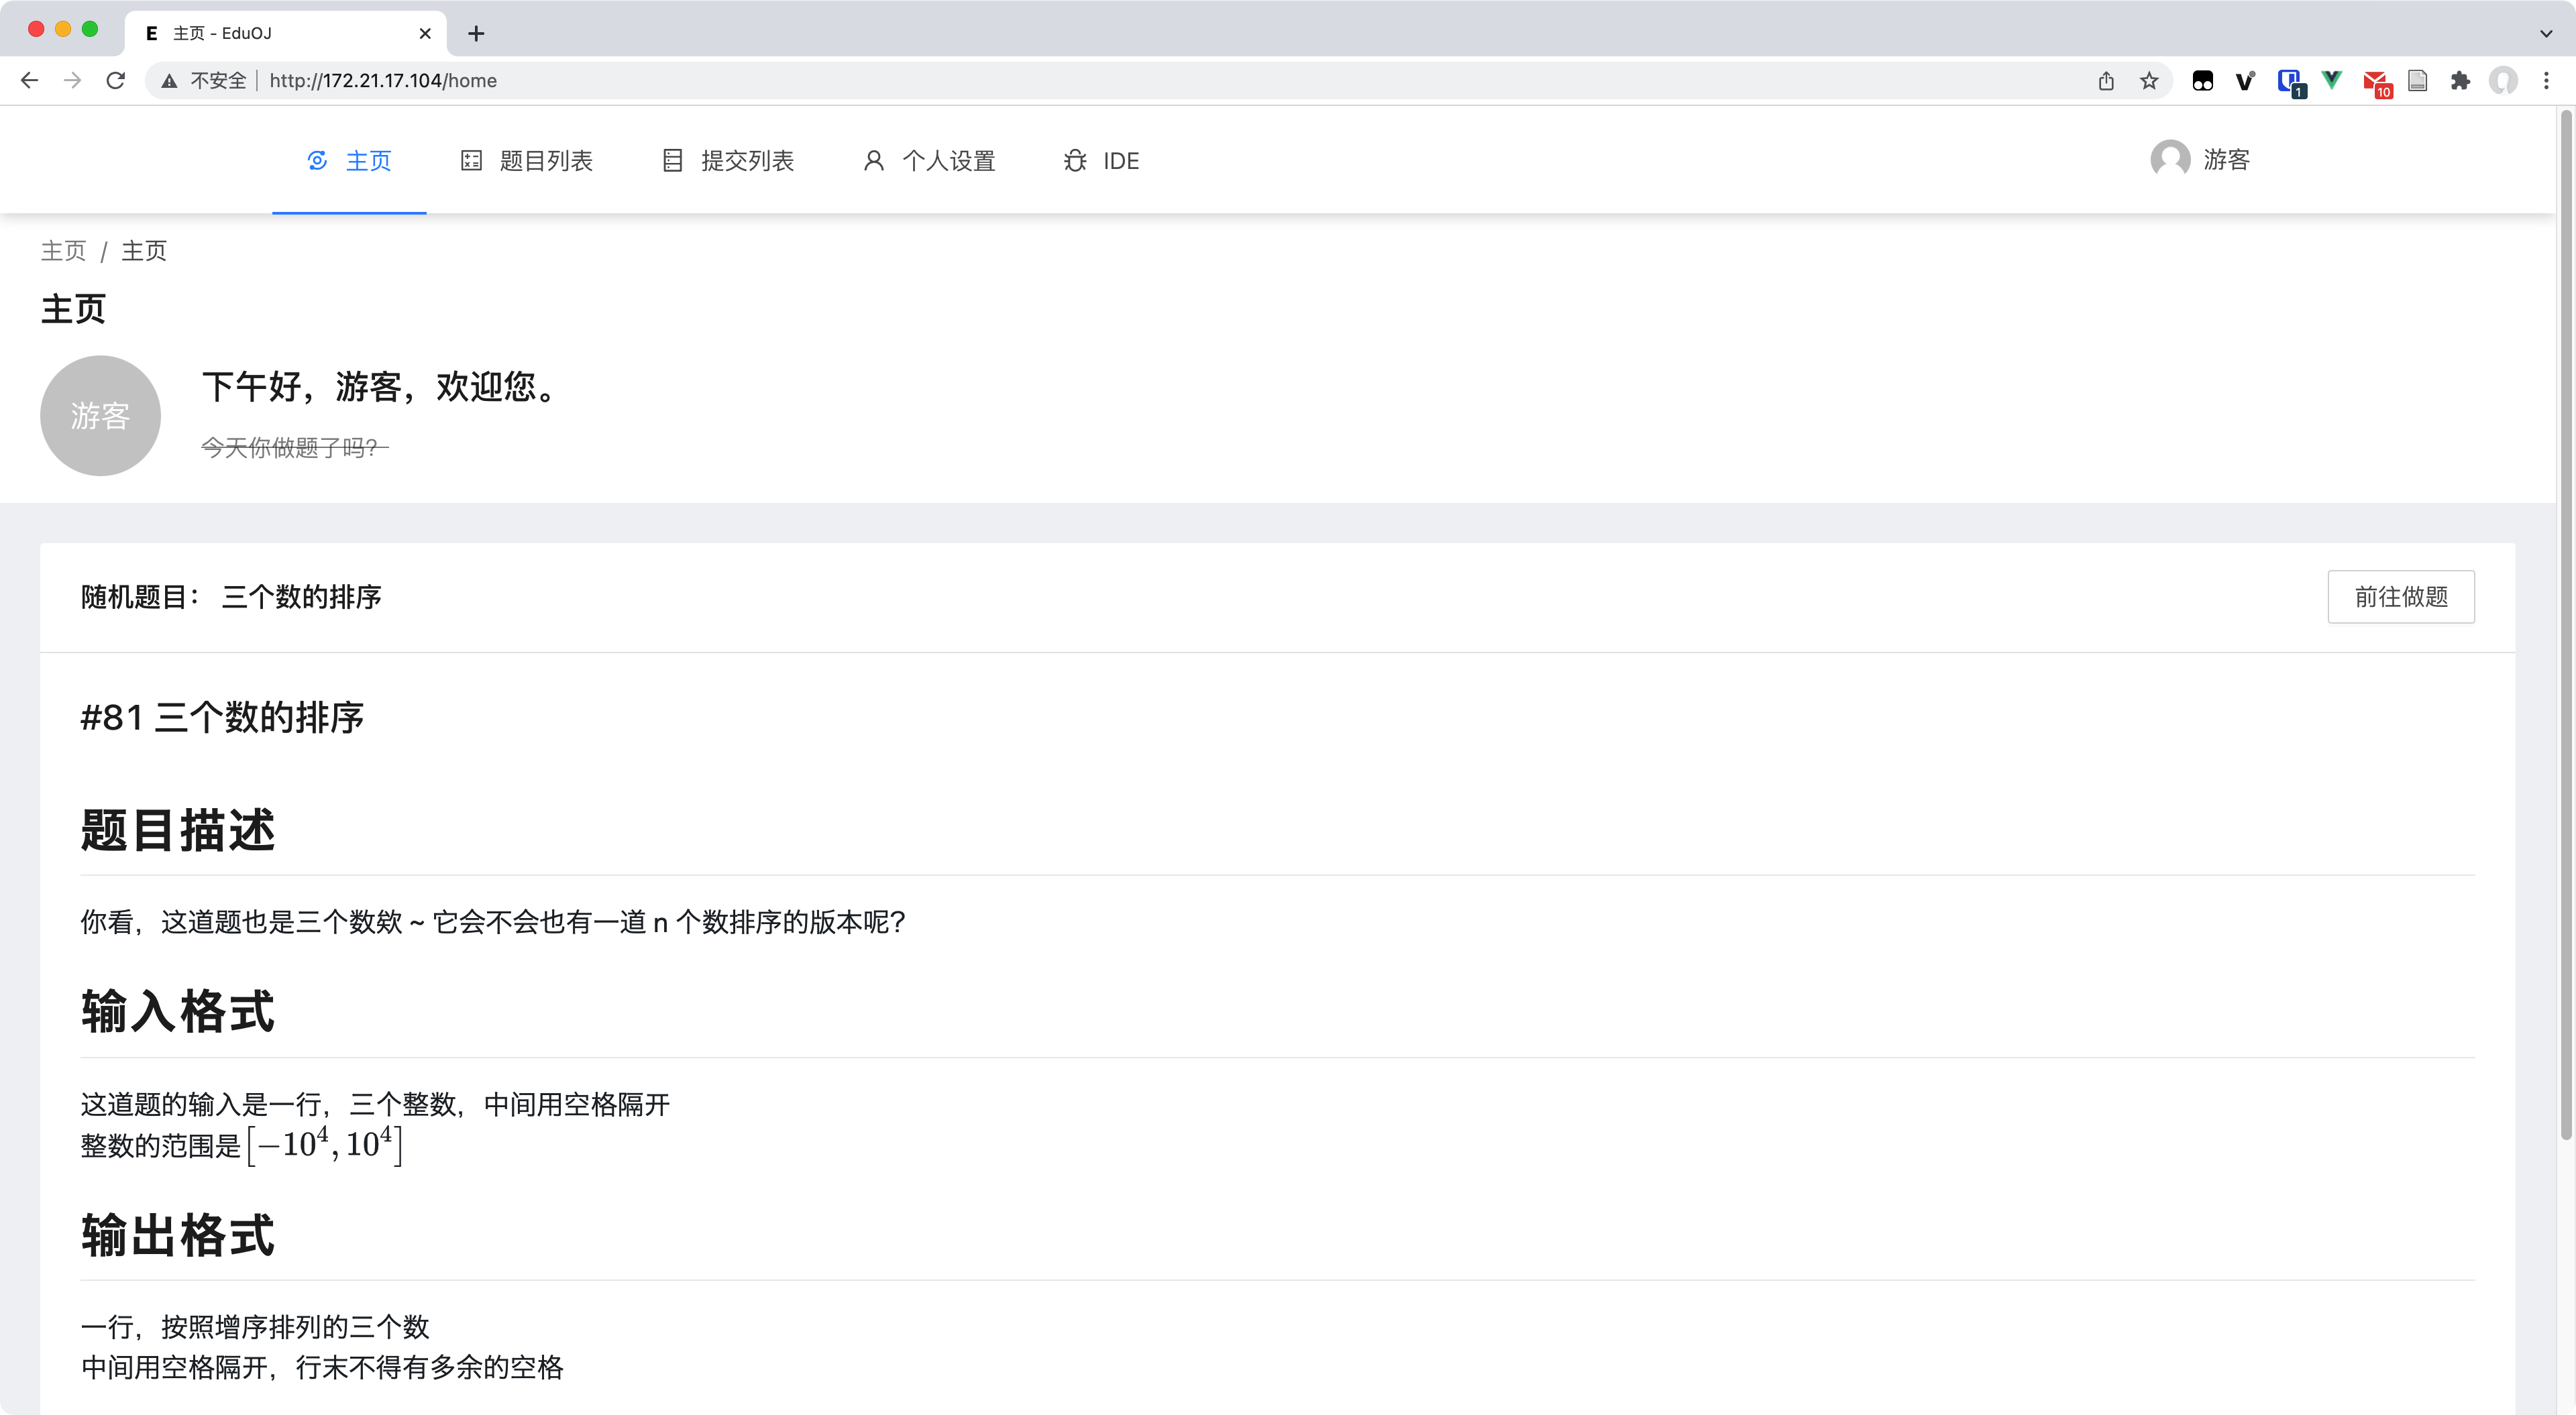
\includegraphics[width=0.8\linewidth]{EduOJ-7.png}
    \caption{EduOJ 游客主页}
\end{figure}
\begin{figure}
    \centering
    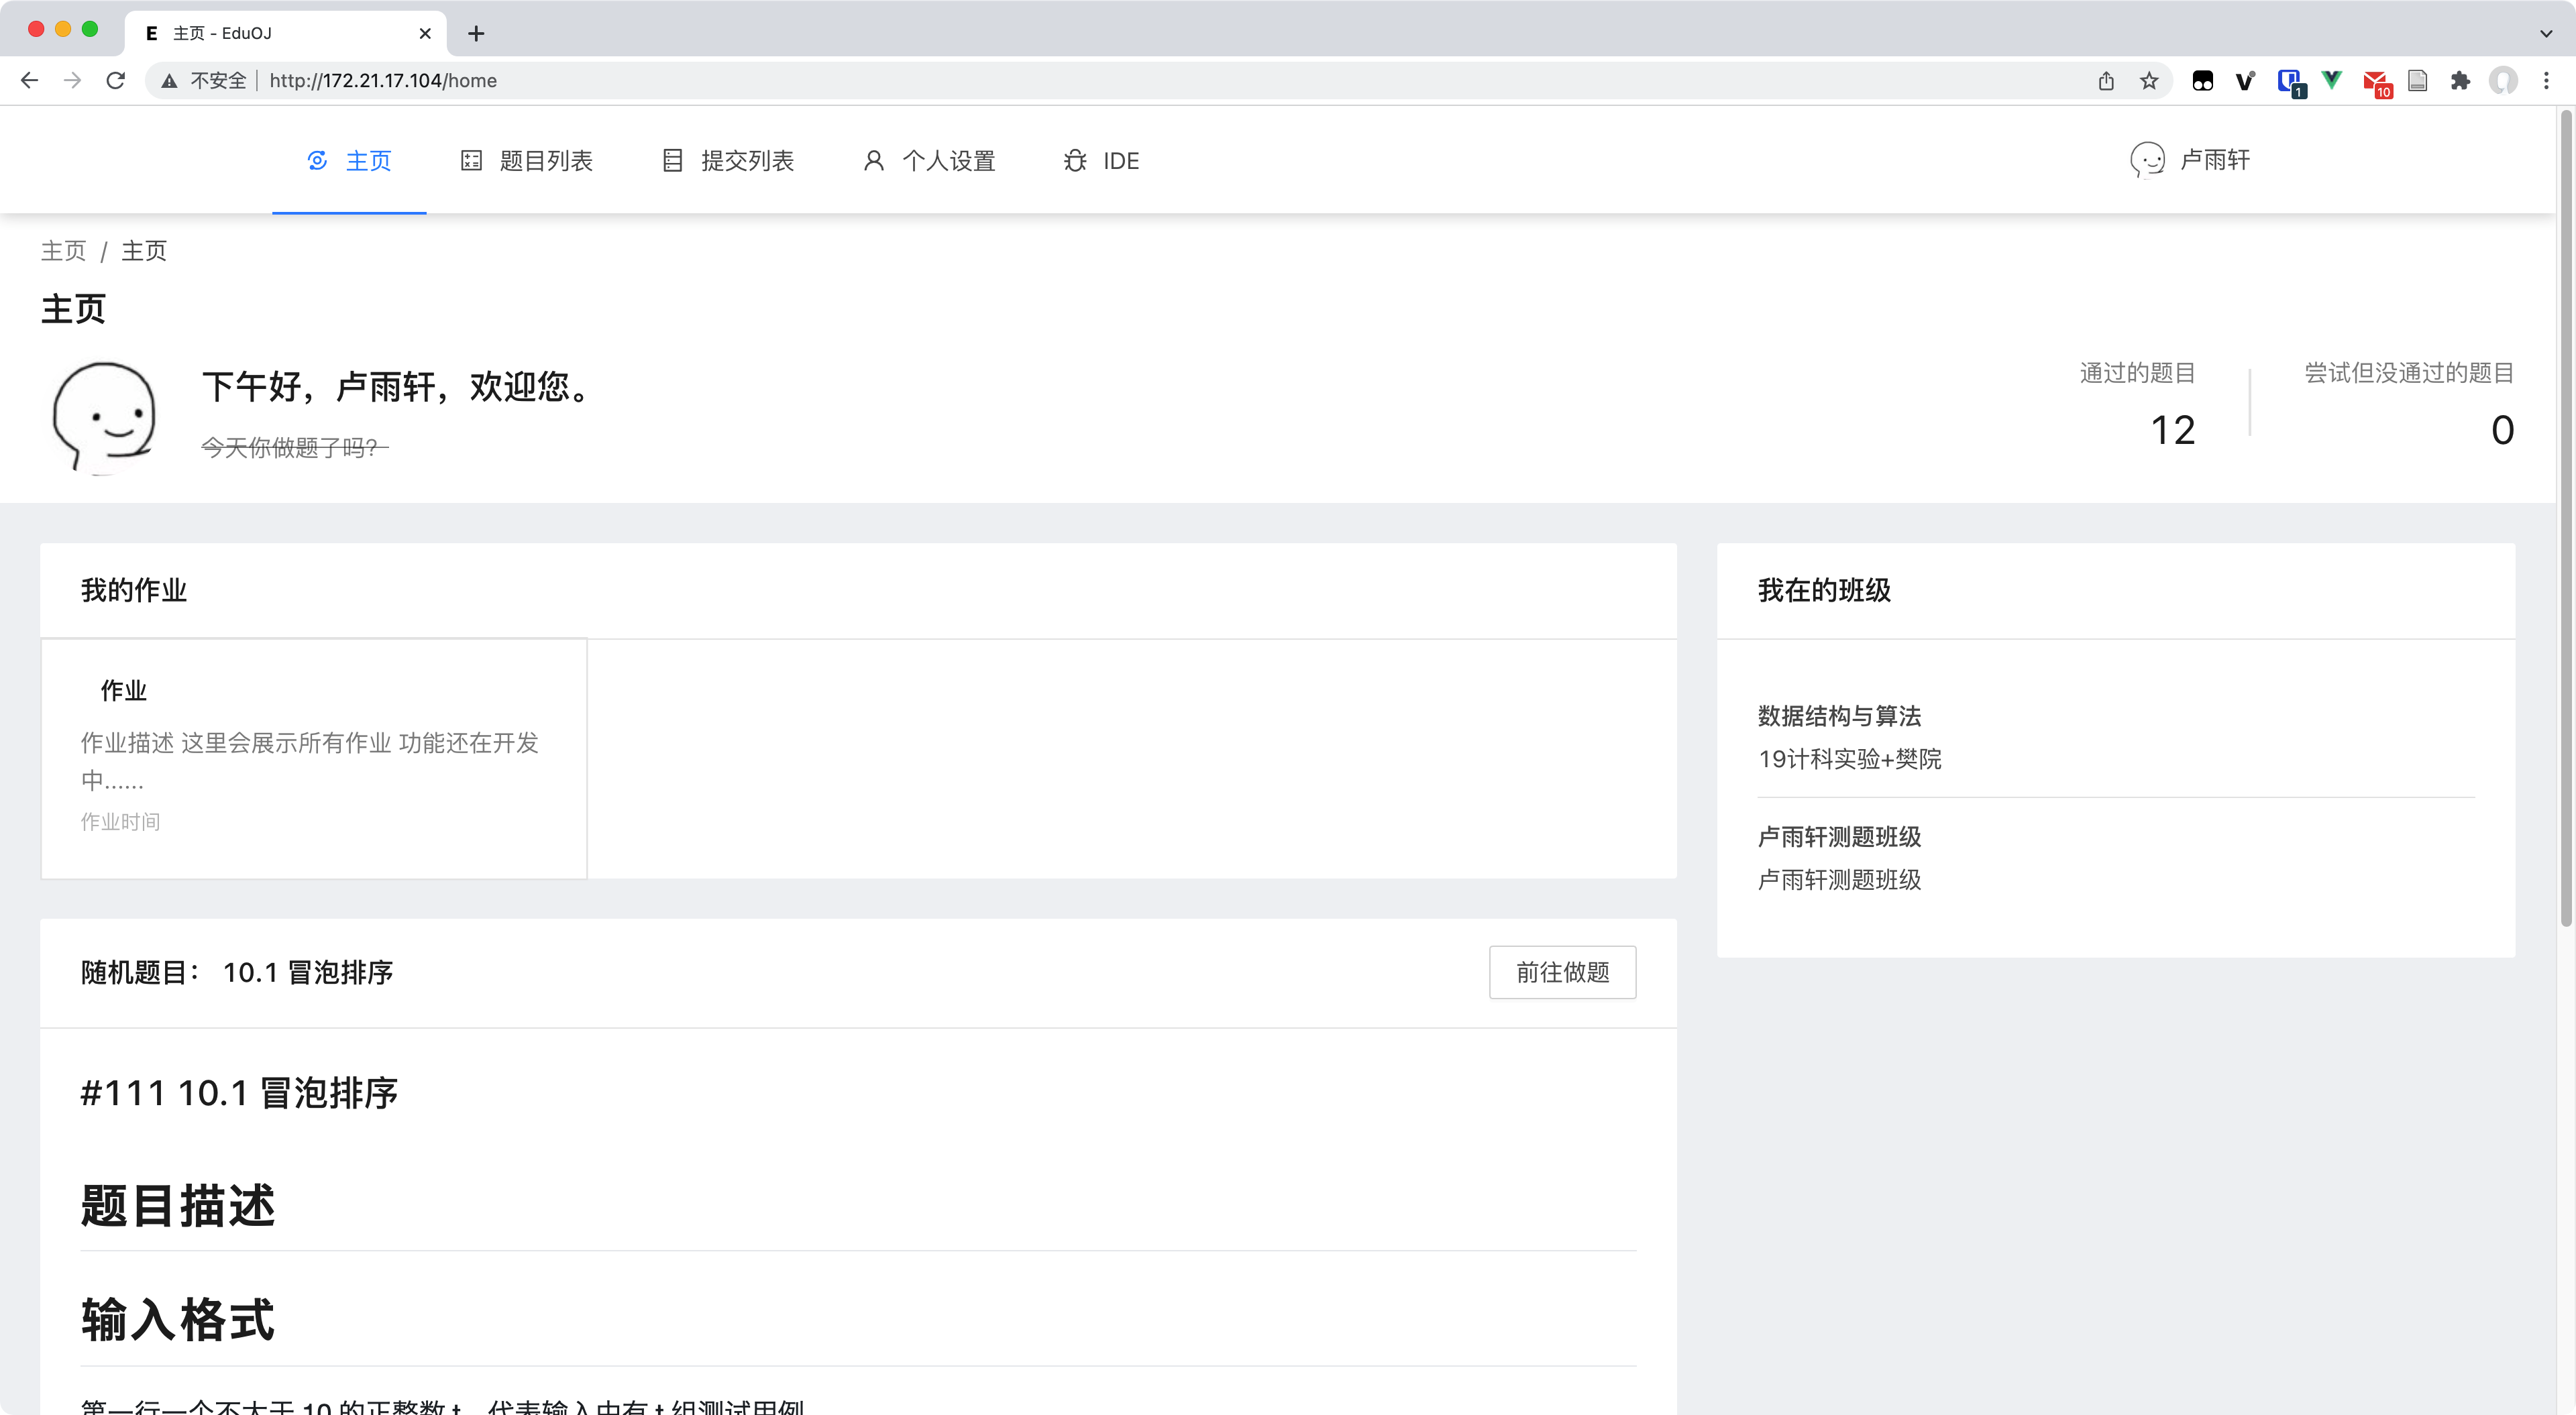
\includegraphics[width=0.8\linewidth]{EduOJ-8.png}
    \caption{EduOJ 用户主页}
\end{figure}

\begin{figure}
    \centering
    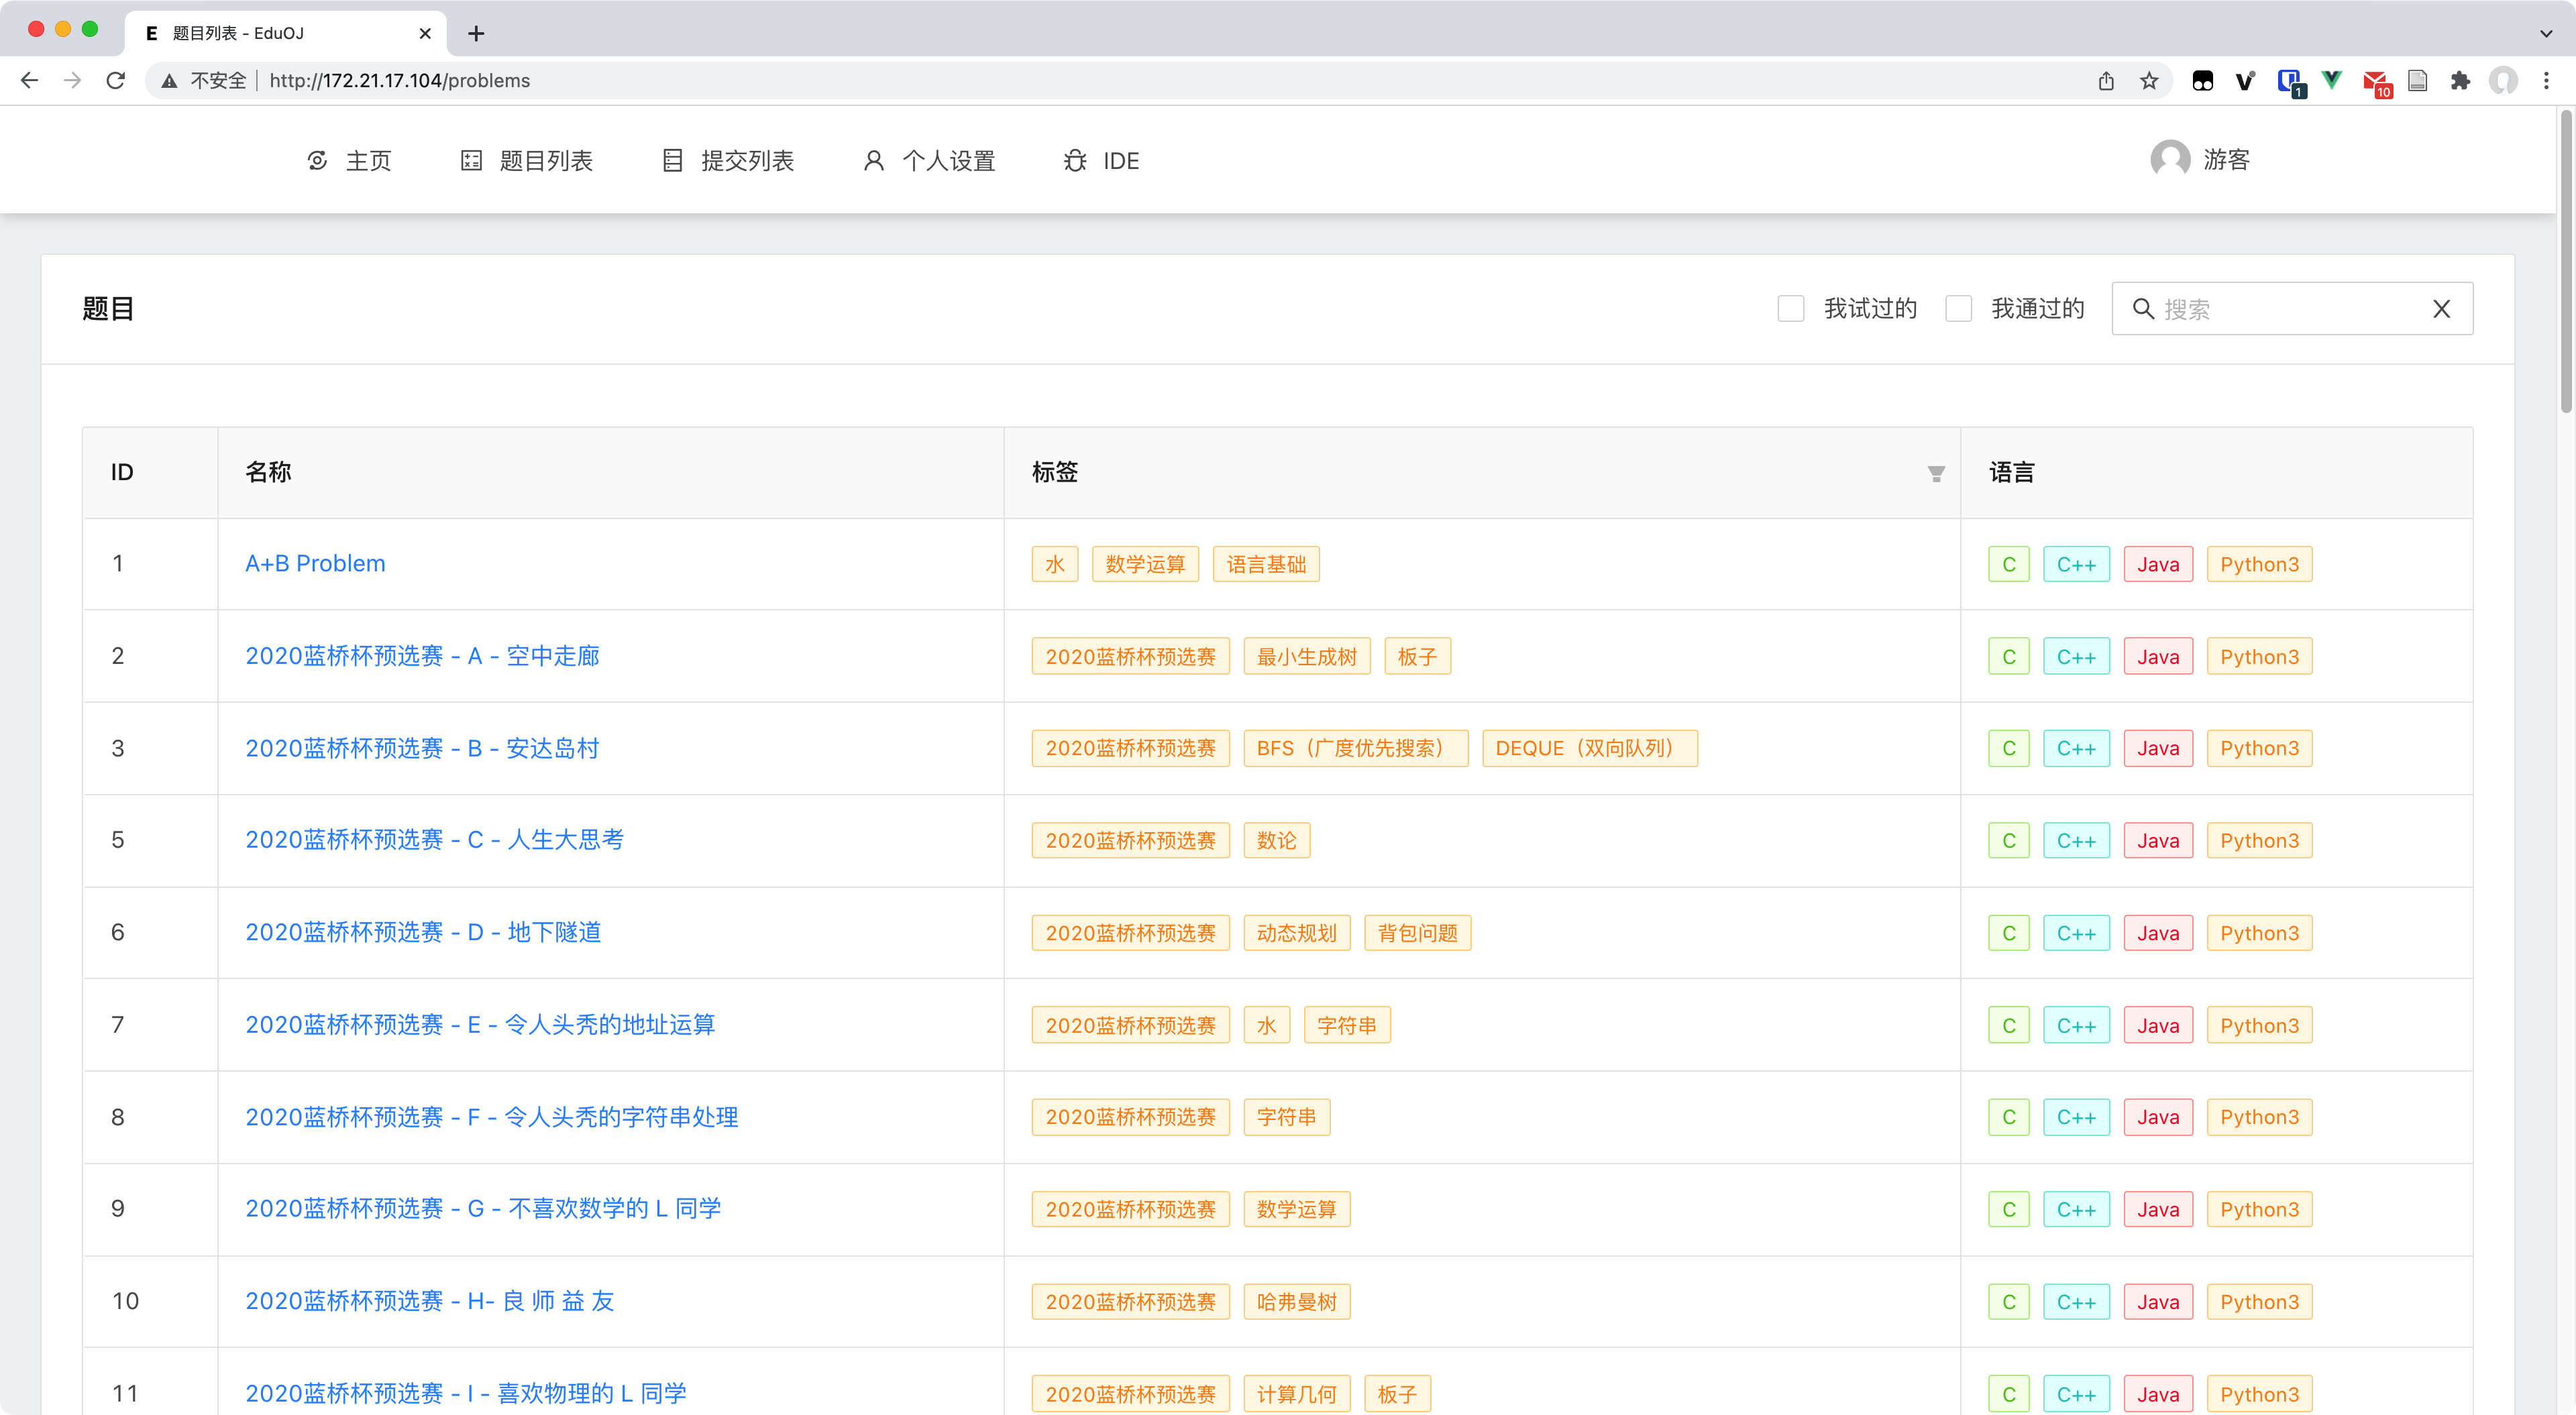
\includegraphics[width=0.8\linewidth]{EduOJ-6.png}
    \caption{EduOJ 题目列表界面}
\end{figure}

\begin{figure}
    \centering
    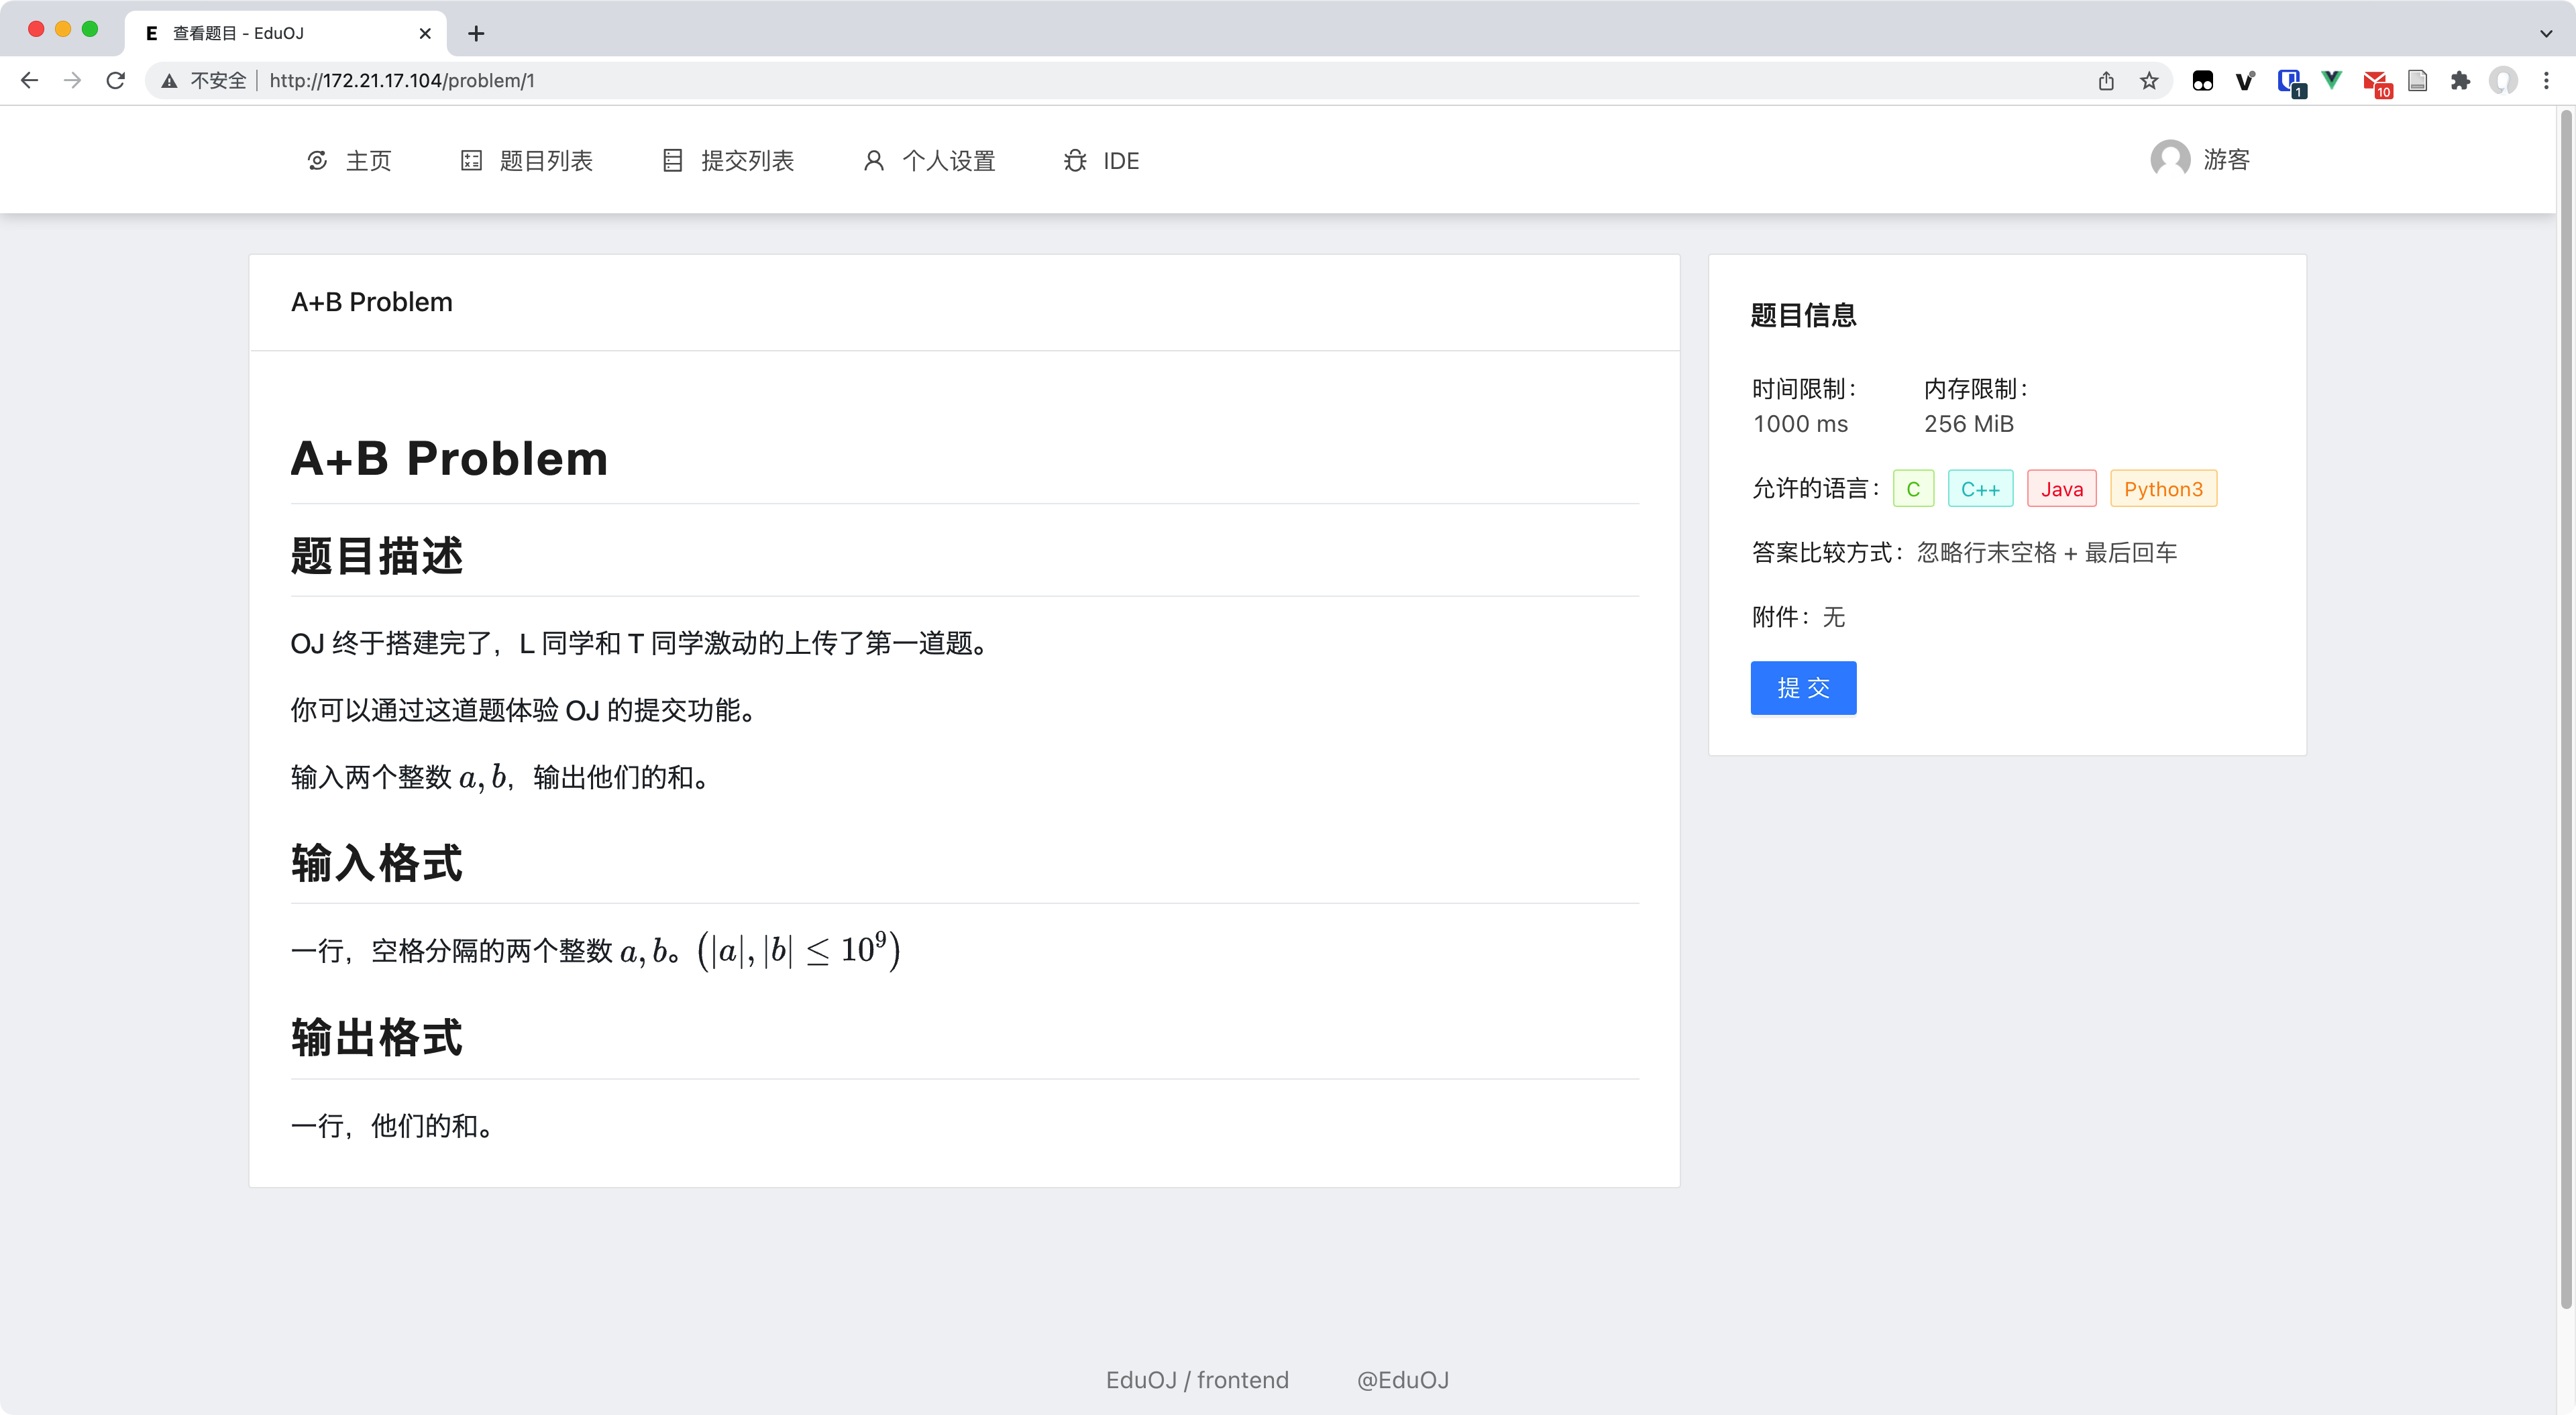
\includegraphics[width=0.8\linewidth]{EduOJ-5.png}
    \caption{EduOJ 查看题目界面}
\end{figure}

\begin{figure}
    \centering
    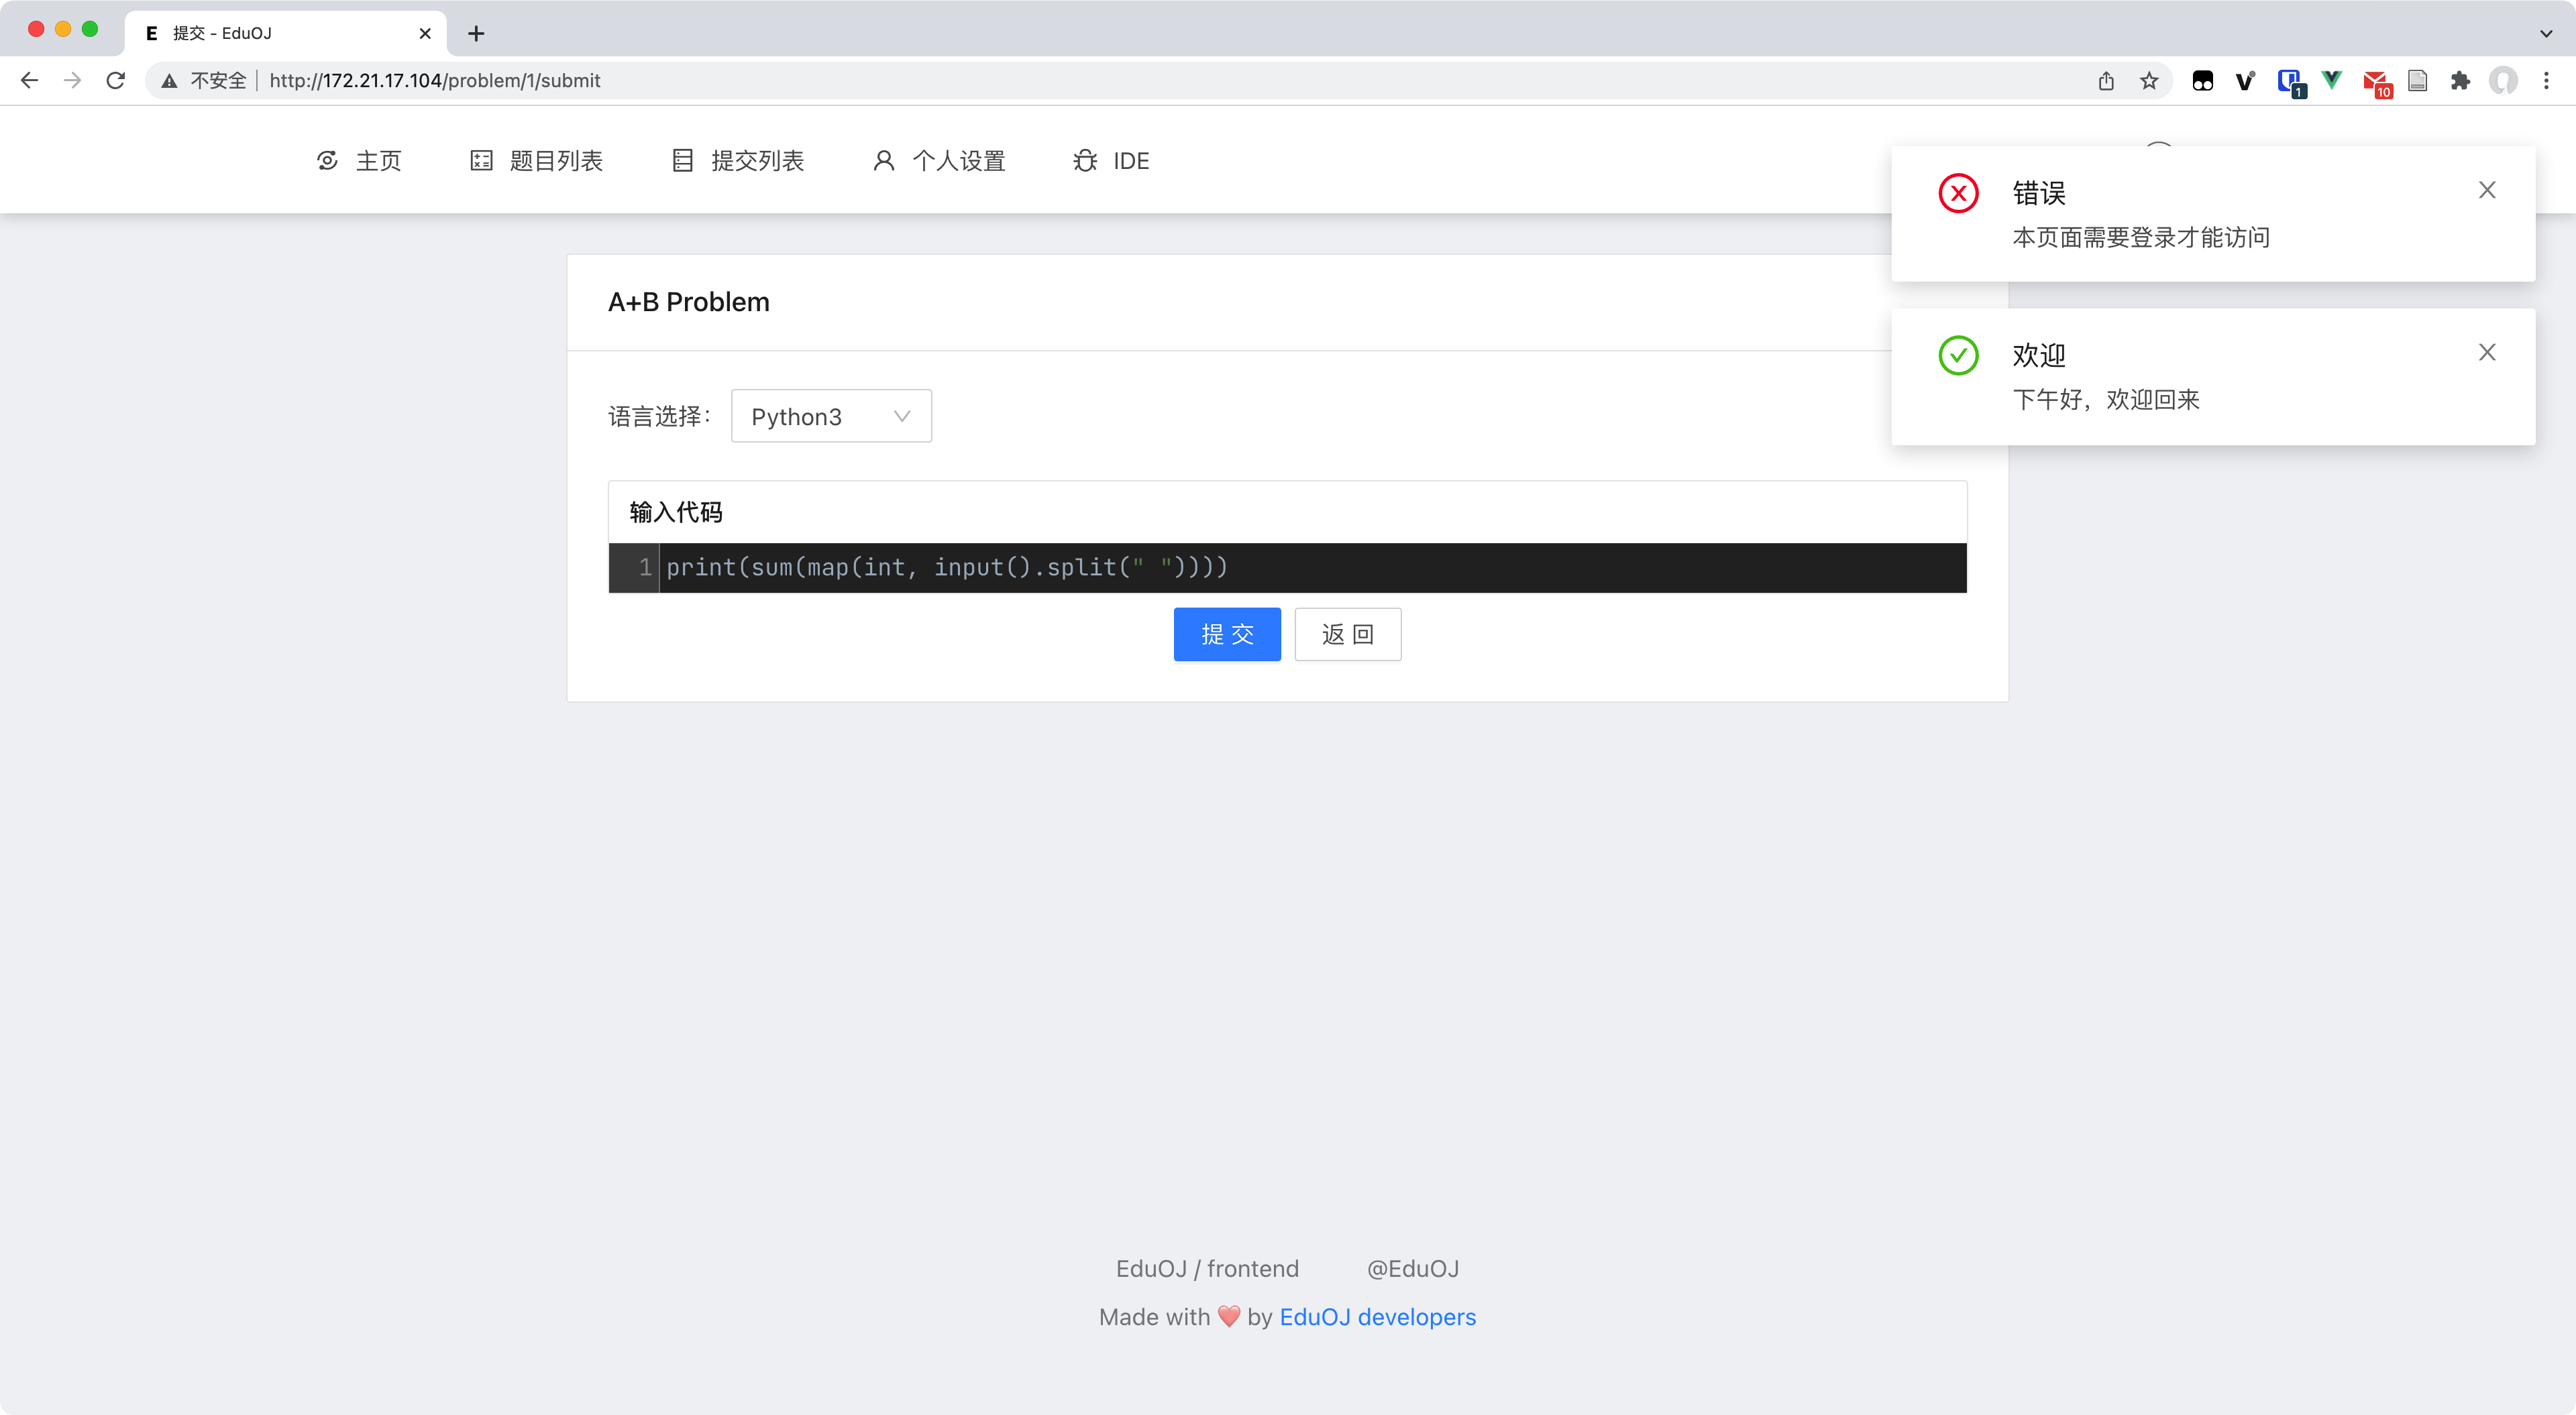
\includegraphics[width=0.8\linewidth]{EduOJ-4.png}
    \caption{EduOJ提交代码界面}
\end{figure}

\begin{figure}
    \centering
    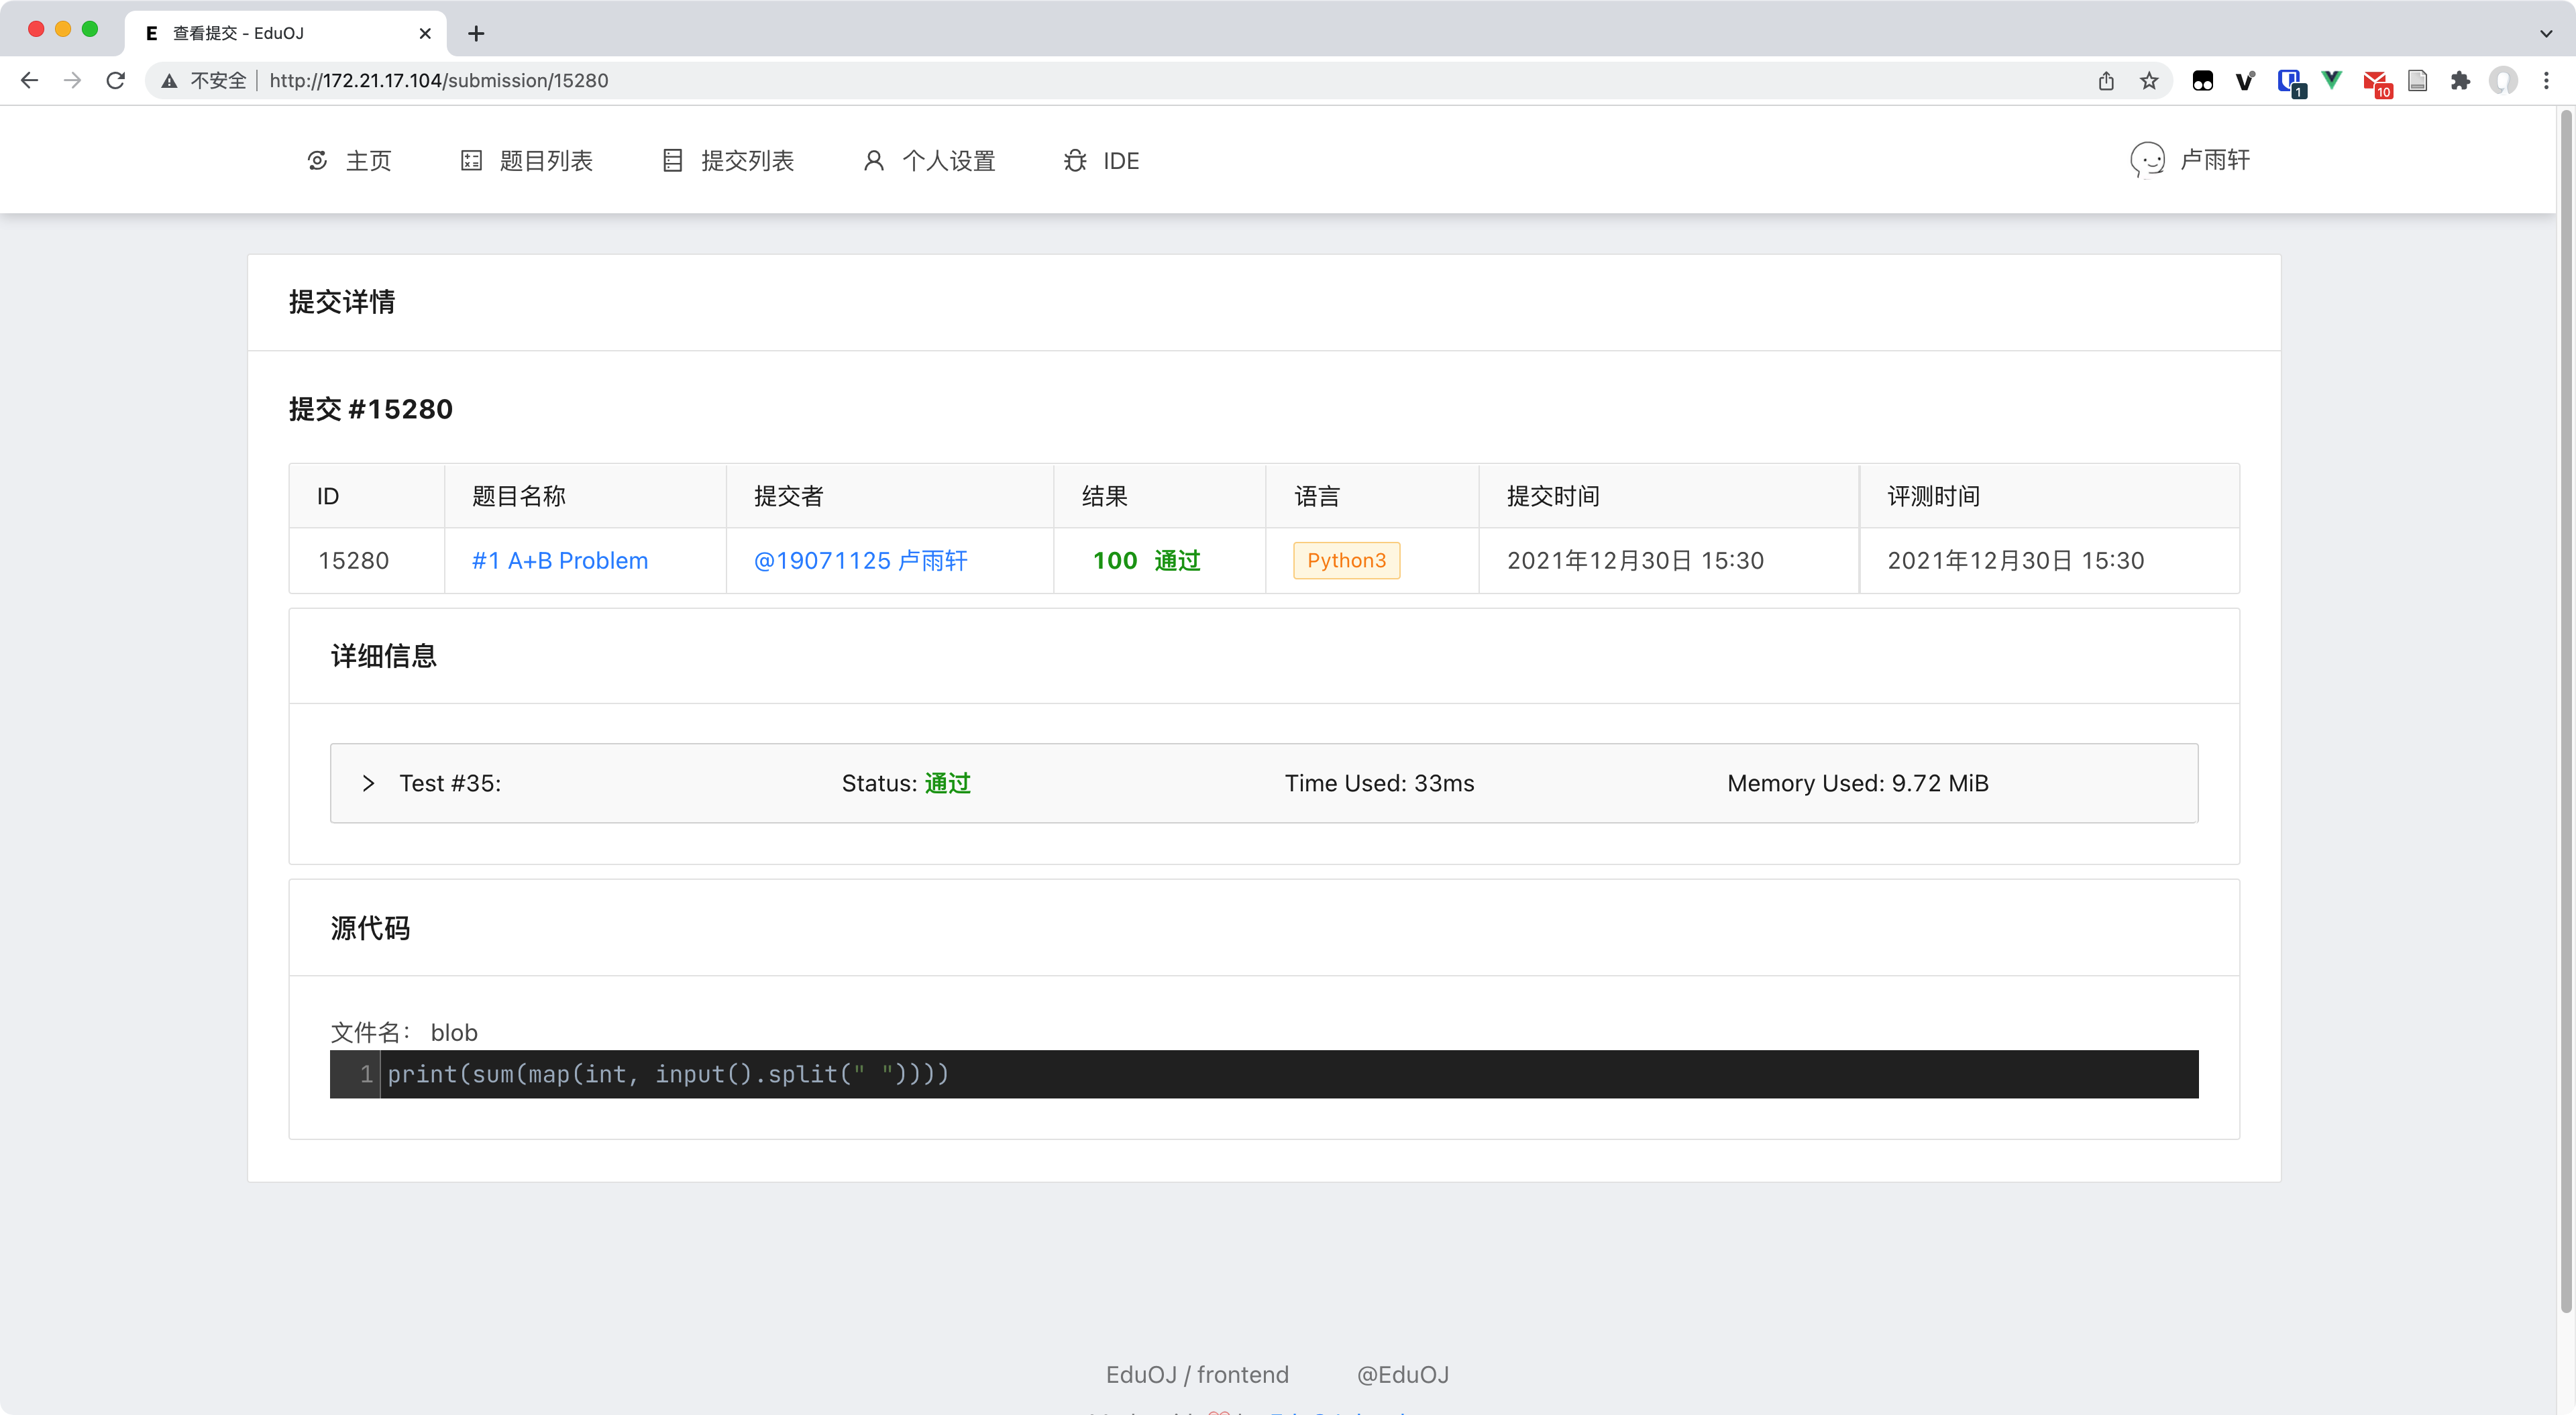
\includegraphics[width=0.8\linewidth]{EduOJ-3.png}
    \caption{EduOJ提交结果界面}
\end{figure}

\begin{figure}
    \centering
    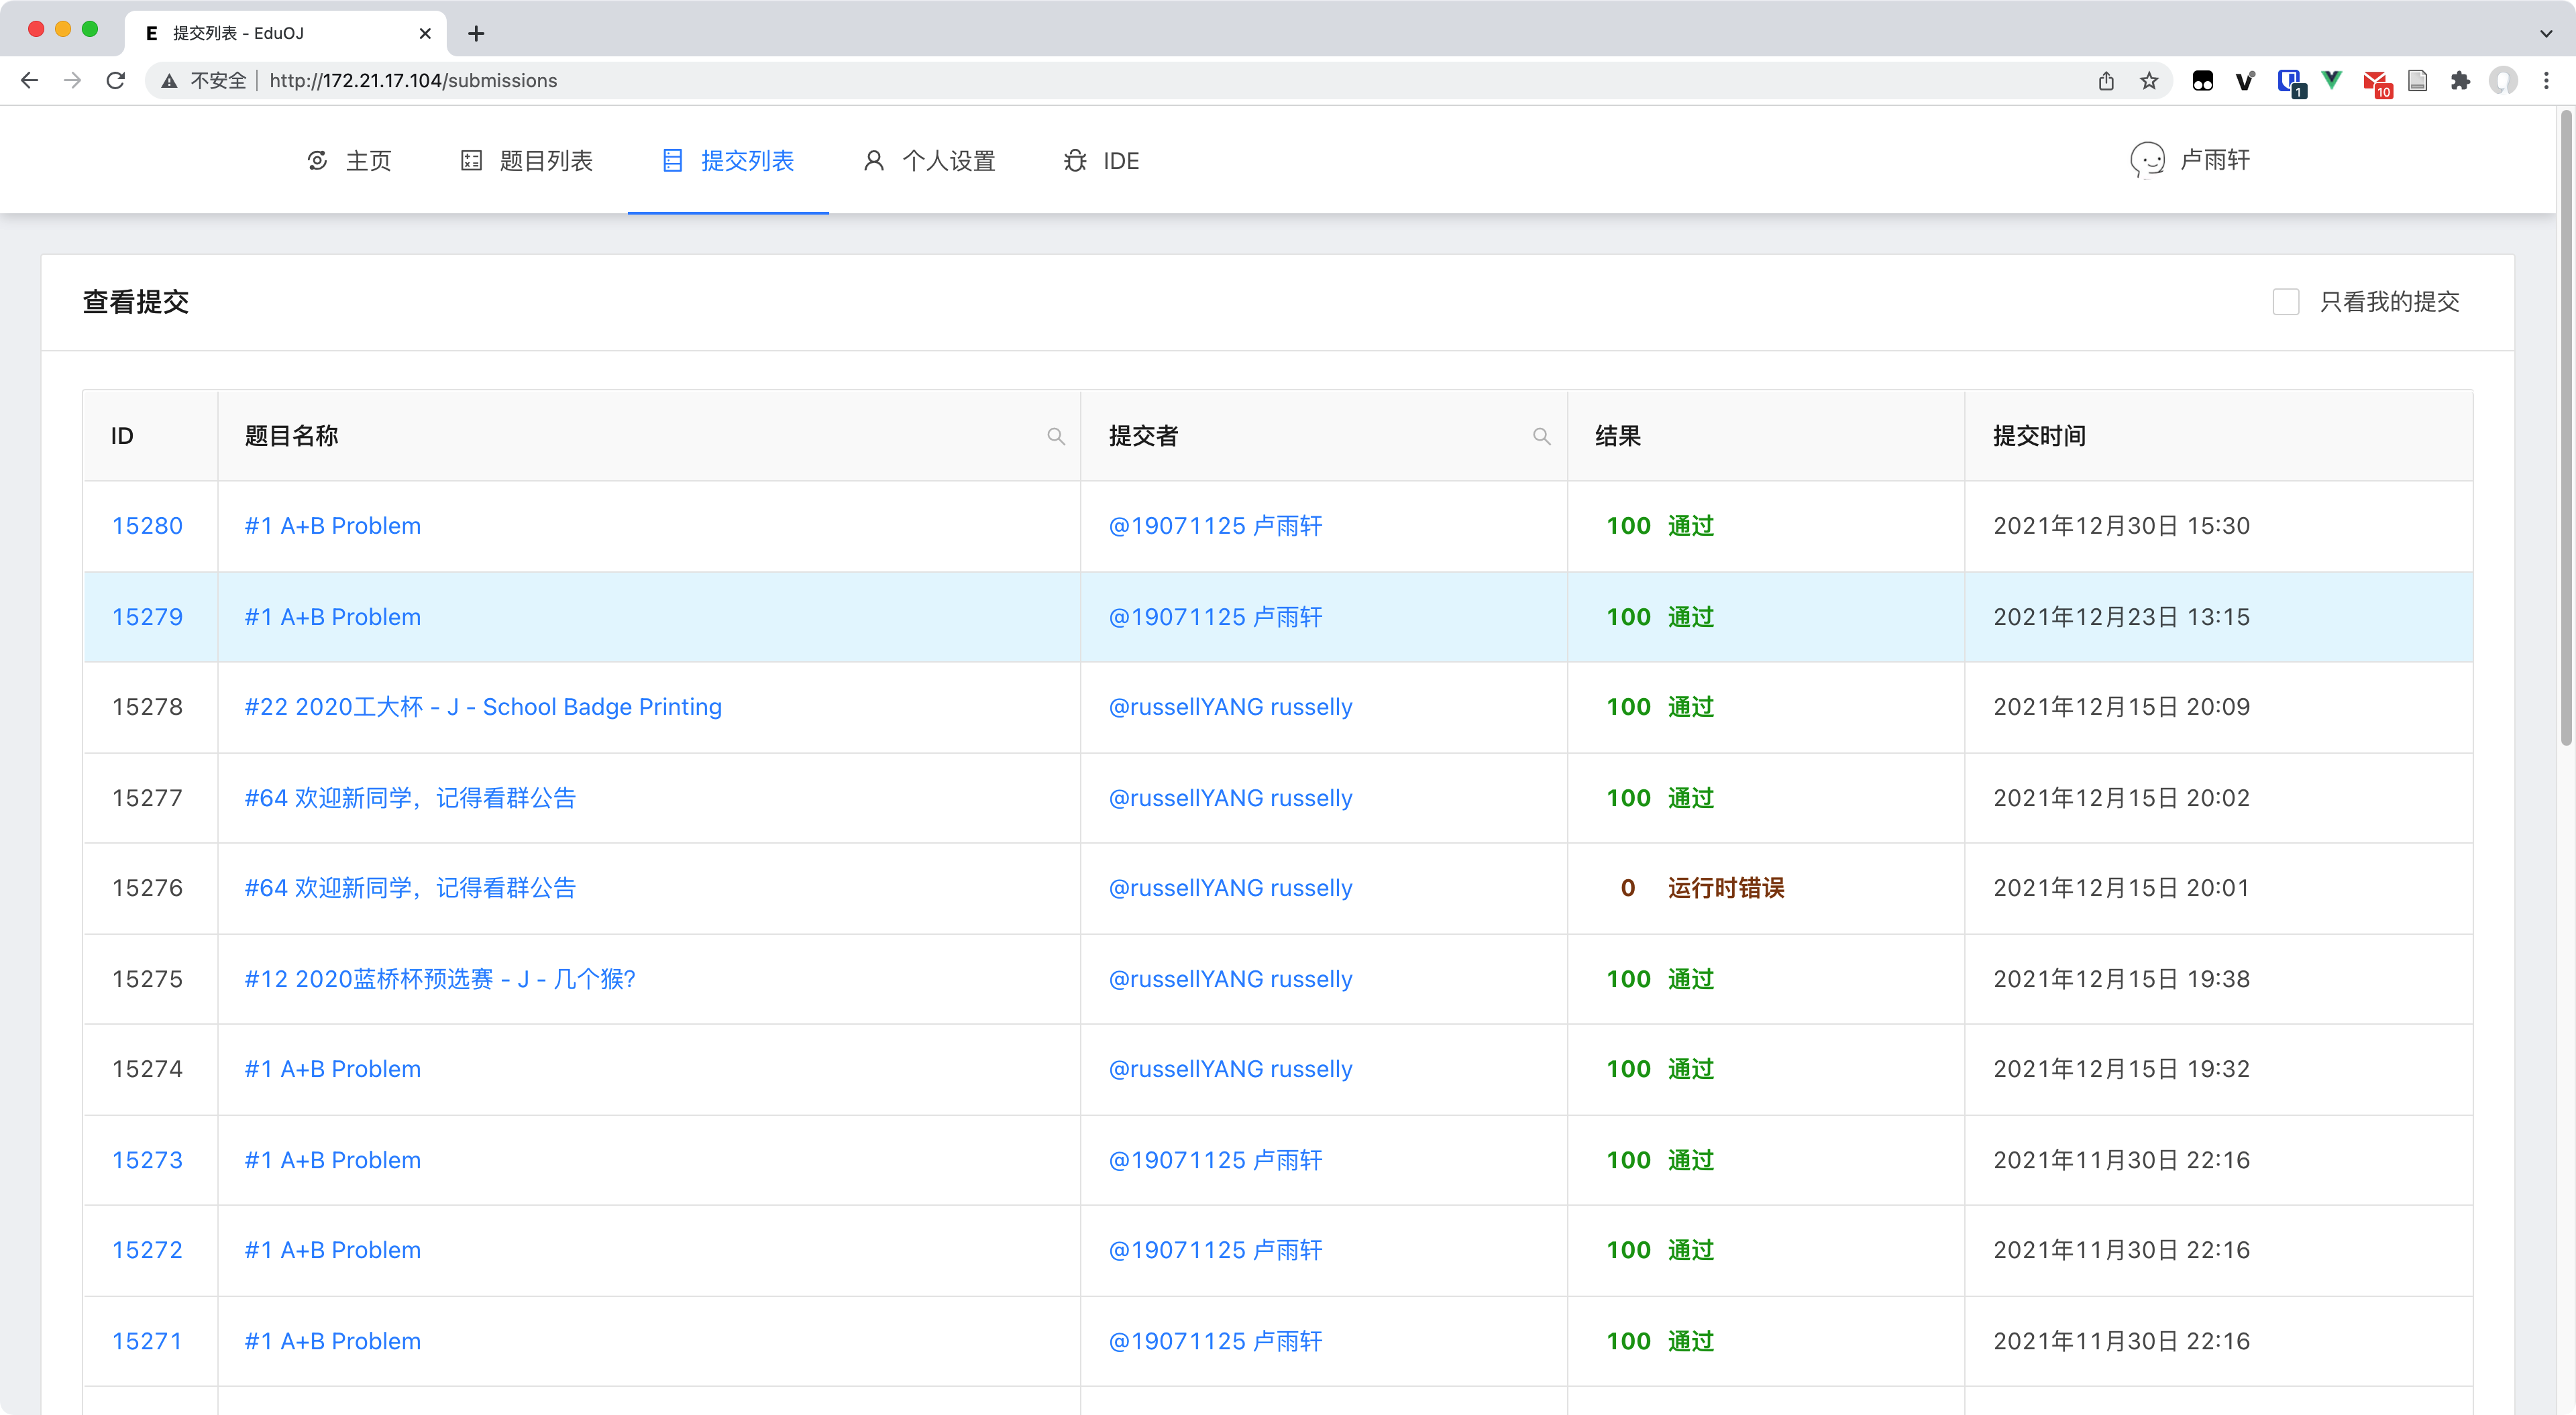
\includegraphics[width=0.8\linewidth]{EduOJ-1.png}
    \caption{EduOJ提交列表界面}
\end{figure}

\begin{figure}
    \centering
    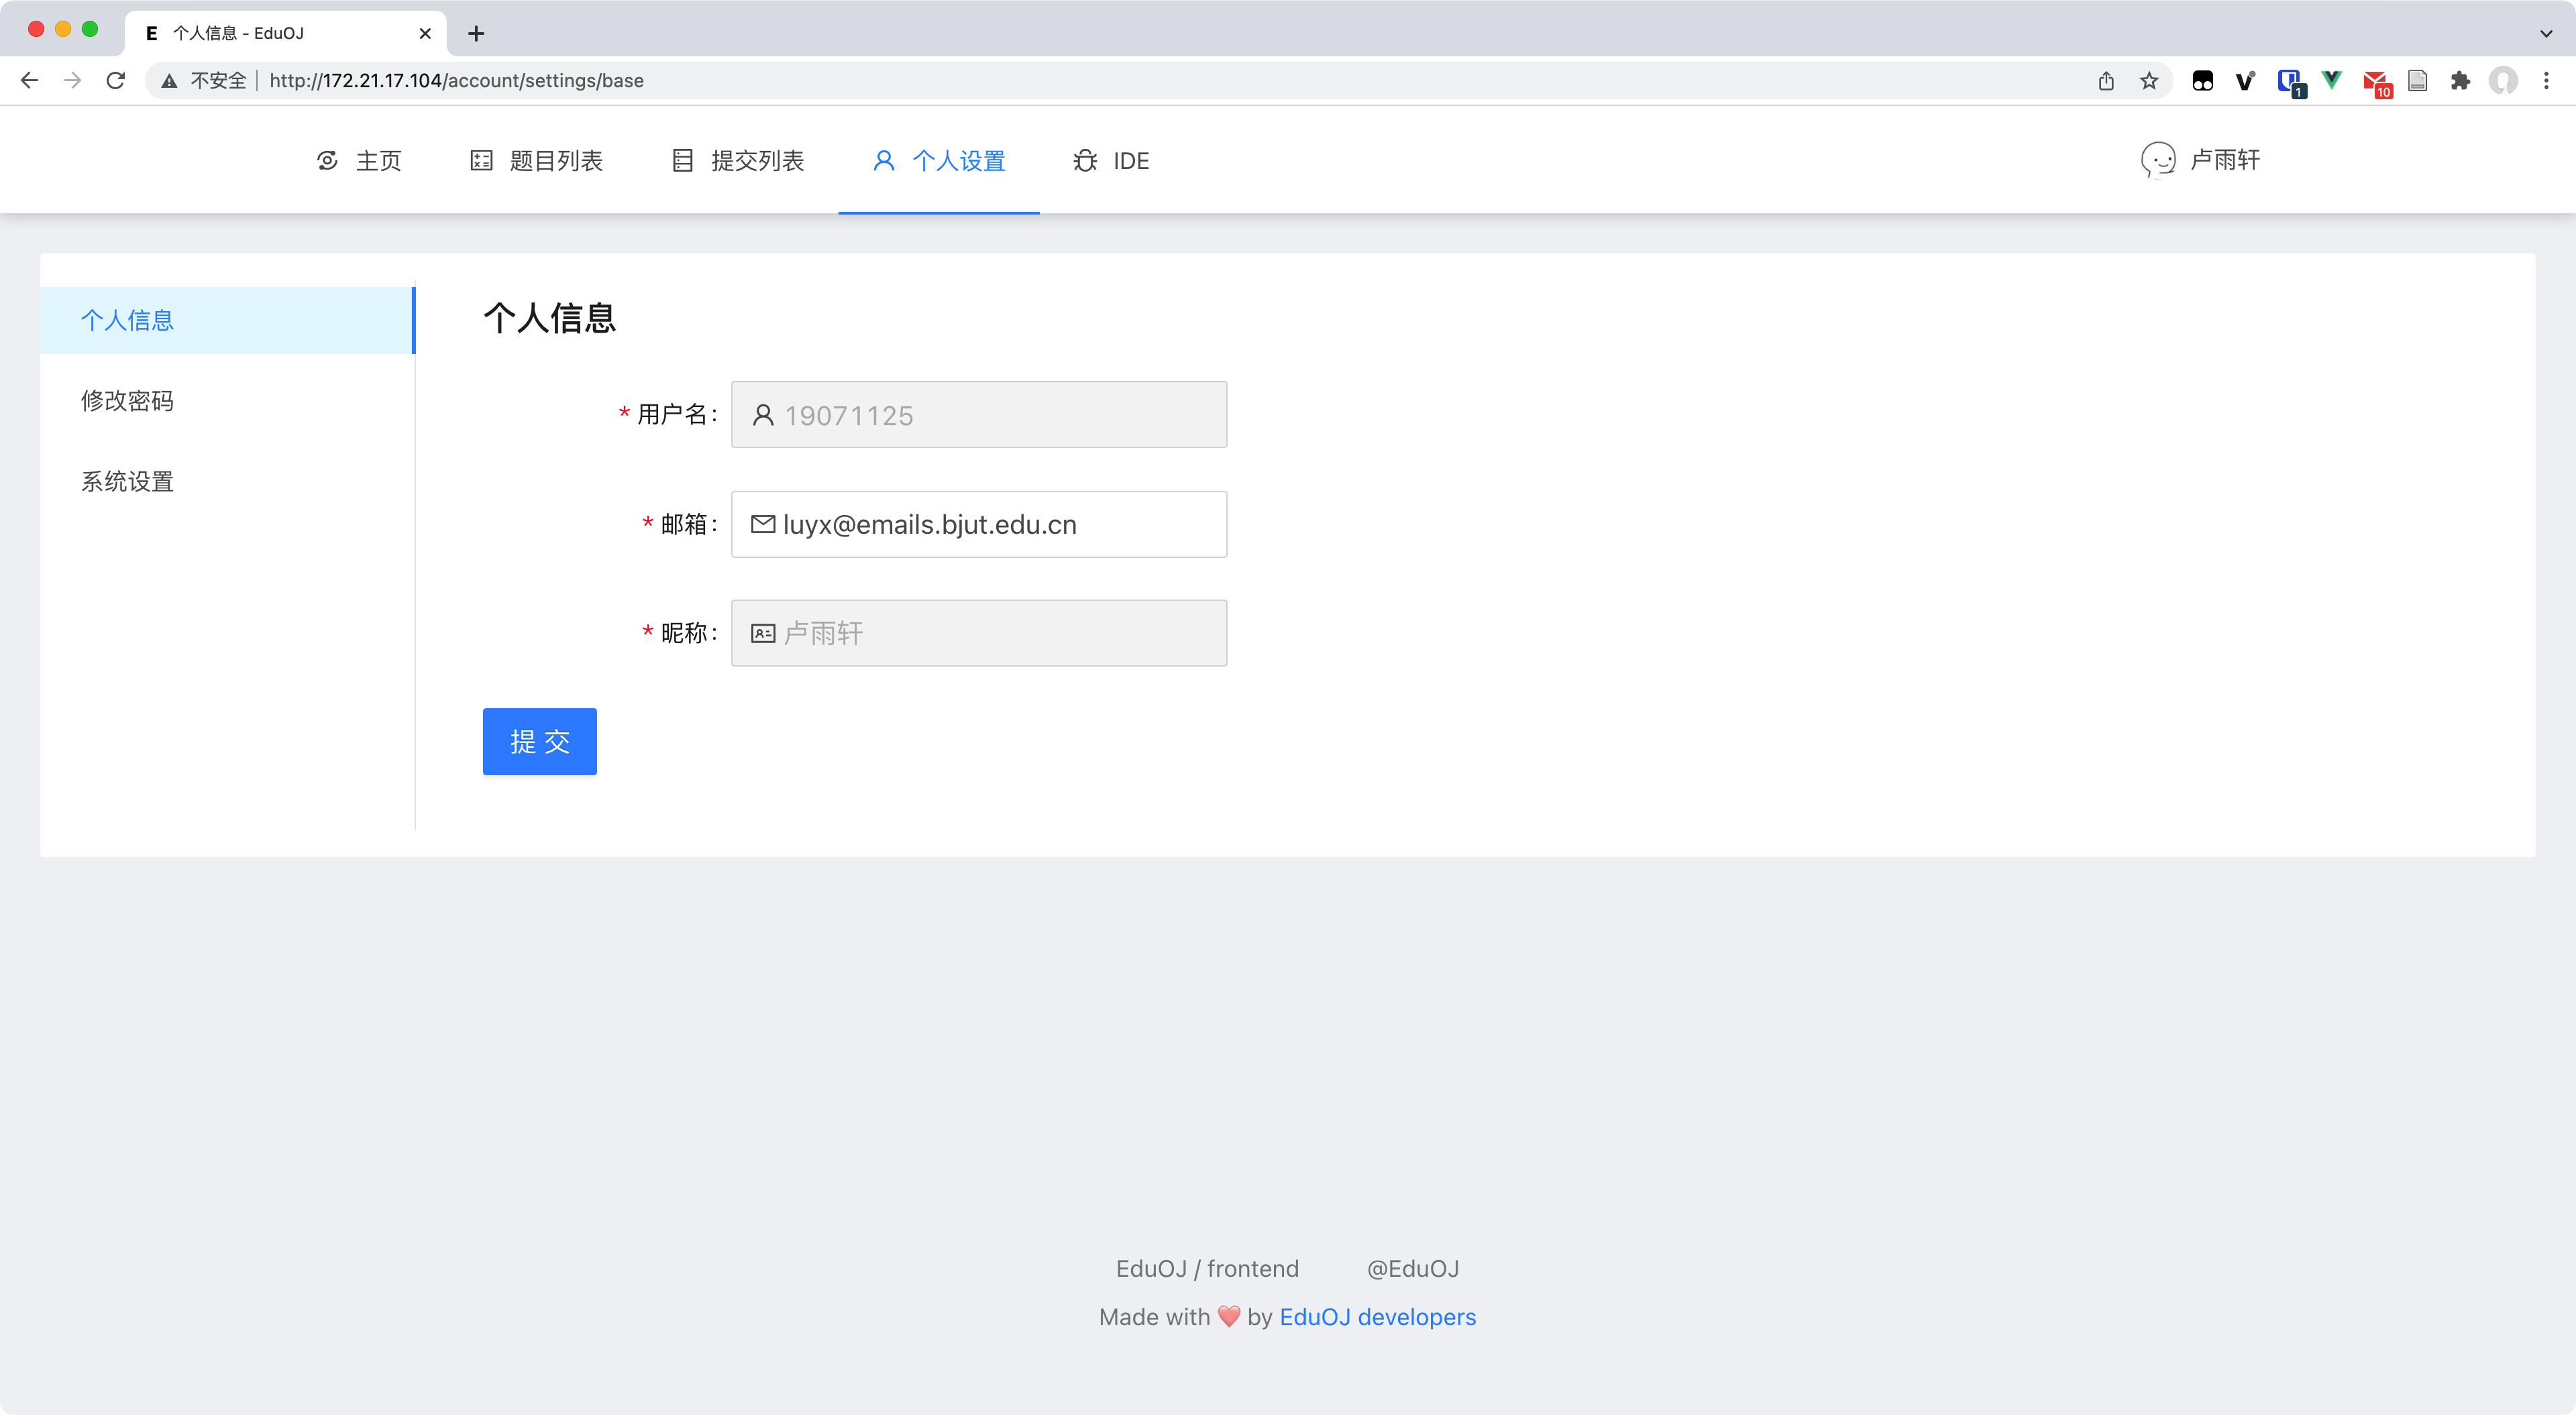
\includegraphics[width=0.8\linewidth]{EduOJ-2.png}
    \caption{EduOJ 个人信息界面}
\end{figure}

\end{appendix}

\end{document}
